%%%%%%%%%%%%%%%%%%%%%%%%%%%%%%%%%%%%%%%%%%%%%%%%%%%%%%%%%%%%%%%%%%%%%%%%%%%%%%%%%%
\begin{frame}[fragile]\frametitle{}
\begin{center}
{\Large Naive Bayes}
\end{center}
\end{frame}

%%%%%%%%%%%%%%%%%%%%%%%%%%%%%%%%%%%%%%%%%%%%%%%%%%%%%%%%%%
\begin{frame}[fragile]\frametitle{Naive Bayes}
 What is it ?
\begin{itemize}
\item Statistical method for classification.
\item Supervised Learning Method.
\item Assumes an underlying probabilistic model, the Bayes theorem.
\item  Can solve problems involving both categorical and continuous valued attributes.
\item  Named after Thomas Bayes, who proposed the Bayes Theorem.
\end{itemize}
\end{frame}


%%%%%%%%%%%%%%%%%%%%%%%%%%%%%%%%%%%%%%%%%%%%%%%%%%%%%%%%%%%
%\begin{frame}[fragile]\frametitle{What we're trying to do}
%\begin{itemize}
%\item Model probabilistic relationships
%\item ``What is the probability that this person will get heart disease, given their diet and workout regimen?''. Output is most similar to Logistic Regression
%\end{itemize}
%\end{frame}
%
%
%%%%%%%%%%%%%%%%%%%%%%%%%%%%%%%%%%%%%%%%%%%%%%%%%%%%%%%%%%%
%\begin{frame}[fragile]\frametitle{What we're trying to do}
%Will introduce Naive Bayes model
%	\begin{itemize}
%	\item A type of Bayesian classifier
%	\item More advanced: Bayesian network
%	\end{itemize}
%\end{frame}

%%%%%%%%%%%%%%%%%%%%%%%%%%%%%%%%%%%%%%%%%%%%%%%%%%%%%%%%%%%
%\begin{frame}[fragile]\frametitle{What we're trying to do}
% Bayes Classifier
%	\begin{itemize}
%	\item A probabilistic framework for solving classification problems
%	\item Used in both naive Bayes and Bayesian networks
%	\item Based on Bayes' Theorem
%	\end{itemize}
%
%\end{frame}

%%%%%%%%%%%%%%%%%%%%%%%%%%%%%%%%%%%%%%%%%%%%%%%%%%%%%%%%%%%%%%%%%%%%%%%%%%%%%%%%%%
\begin{frame}[fragile]\frametitle{}
\begin{center}
{\Large Bayes Theorem}
\end{center}
\end{frame}


%%%%%%%%%%%%%%%%%%%%%%%%%%%%%%%%%%%%%%%%%%%%%%%%%%%%%%%%%%
\begin{frame}[fragile]\frametitle{Probability (recap): Single (Marginal) Probability}
\begin{itemize}
\item A random variable $X$ is just something whose value isn't fixed in advance: rolling a die, tomorrow's weather, whether a message is spam.
\item $P(X=x)$ is the probability that $X$ takes one particular value $x$, ignoring every other variable in the problem entirely; that's why it's also called the \textbf{marginal} probability.
\item Example: for a fair die, $P(X=6) = 1/6$. For weather, $P(\text{Rain}) = 0.3$ describes rain on its own, nothing else.
\item Shorthand: $P(X)$ (without ``$=x$'') usually means ``the whole distribution over every value $X$ can take''; $P(X=x)$ pins it to one specific value.
\end{itemize}
\begin{center}
\begin{adjustbox}{max width=\linewidth}
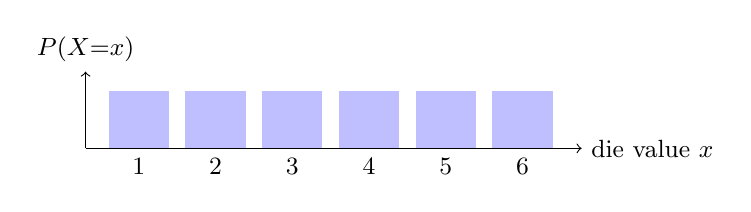
\begin{tikzpicture}[scale=0.75]
\filldraw[blue!25] (0,0) rectangle (1,0.96);
\filldraw[blue!25] (1.3,0) rectangle (2.3,0.96);
\filldraw[blue!25] (2.6,0) rectangle (3.6,0.96);
\filldraw[blue!25] (3.9,0) rectangle (4.9,0.96);
\filldraw[blue!25] (5.2,0) rectangle (6.2,0.96);
\filldraw[blue!25] (6.5,0) rectangle (7.5,0.96);
\node[below] at (0.5,0) {\small 1};
\node[below] at (1.8,0) {\small 2};
\node[below] at (3.1,0) {\small 3};
\node[below] at (4.4,0) {\small 4};
\node[below] at (5.7,0) {\small 5};
\node[below] at (7.0,0) {\small 6};
\draw[->] (-0.4,0) -- (8.0,0) node[right]{\small die value $x$};
\draw[->] (-0.4,0) -- (-0.4,1.3) node[above]{\small $P(X{=}x)$};
\end{tikzpicture}
\end{adjustbox}
\vspace{2mm}

{\small Each face of a fair die is equally likely: $P(X=x)=1/6$ for every $x$.}
\end{center}
\end{frame}

%%%%%%%%%%%%%%%%%%%%%%%%%%%%%%%%%%%%%%%%%%%%%%%%%%%%%%%%%%
\begin{frame}[fragile]\frametitle{Probability (recap): Joint Probability}
\begin{itemize}
\item Joint probability: ``$X$ and $Y$'', written $P(X=x, Y=y)$ or just $P(X,Y)$.
  \begin{itemize}
  \item In plain English: the probability that variable $X$ takes on the value $x$ \emph{and} variable $Y$ has the value $y$, both at once: the same statement, just spelled out.
  \end{itemize}
\item Example: $X$ = Weather (Rain or not), $Y$ = Carrying an umbrella (Yes or No). $P(\text{Rain}, \text{Umbrella}{=}\text{Yes})$ is the chance both happen together.
\end{itemize}
\begin{center}
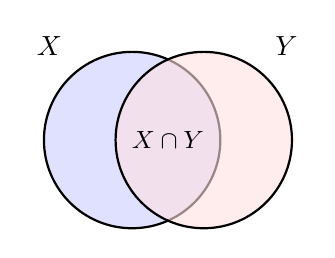
\begin{tikzpicture}[scale=0.7]
\draw[thick,fill=blue!12] (0,0.6) circle (1.6);
\draw[thick,fill=red!12,fill opacity=0.6] (1.3,0.6) circle (1.6);
\node at (-1.5,2.3) {\normalsize $X$};
\node at (2.8,2.3) {\normalsize $Y$};
\node[align=center] at (0.65,0.6) {\small $X\cap Y$};
\end{tikzpicture}

{\small \textbf{Joint} $P(X,Y)$: the overlap region, everything that is in both circles at once.}
\end{center}
\end{frame}

%%%%%%%%%%%%%%%%%%%%%%%%%%%%%%%%%%%%%%%%%%%%%%%%%%%%%%%%%%
\begin{frame}[fragile]\frametitle{Probability (recap): Independence}
\begin{itemize}
\item Two variables are \textbf{independent} if knowing the value of one tells you nothing about the other.
\item Then the joint probability is simply the product: $P(X,Y) = P(X)\times P(Y)$.
\item Example: two separate coin flips. $P(\text{1st}{=}H) = 0.5$ and $P(\text{2nd}{=}H)=0.5$; since the coins don't affect each other, $P(\text{both}{=}H) = 0.5\times0.5=0.25$, and as the grid below shows, that's exactly one of four equally likely outcomes.
\item This is the assumption Naive Bayes leans on heavily (features assumed independent given the class); we'll return to it soon.
\end{itemize}
\begin{center}
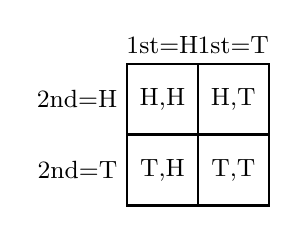
\begin{tikzpicture}[scale=0.9]
\draw[thick] (0,0) rectangle (2,2);
\draw[thick] (0,1) -- (2,1);
\draw[thick] (1,0) -- (1,2);
\node at (0.5,1.5) {\small H,H};
\node at (1.5,1.5) {\small H,T};
\node at (0.5,0.5) {\small T,H};
\node at (1.5,0.5) {\small T,T};
\node[above] at (0.5,2) {\small 1st=H};
\node[above] at (1.5,2) {\small 1st=T};
\node[left] at (0,1.5) {\small 2nd=H};
\node[left] at (0,0.5) {\small 2nd=T};
\end{tikzpicture}

{\small Each of the 4 cells is equally likely: $0.25$, exactly $P(1\text{st})\times P(2\text{nd})$.}
\end{center}
\end{frame}

%%%%%%%%%%%%%%%%%%%%%%%%%%%%%%%%%%%%%%%%%%%%%%%%%%%%%%%%%%
\begin{frame}[fragile]\frametitle{Probability (recap): Conditional Probability}
\begin{itemize}
\item Conditional probability: ``$Y$'' given that we've already observed ``$X$'': $P(Y=y|X=x)$, shorthand $P(Y|X)$.
\item Better way to understand it: restrict your attention to only the $X=x$ world (forget everything outside it), then ask how much of that restricted world is also $Y=y$.
\item Formally, $P(Y|X) = \dfrac{P(X,Y)}{P(X)}$: the joint overlap, as a fraction of $X$ alone, not of everything.
\item Example: of all rainy days, what fraction did the person carry an umbrella? That's $P(\text{Umbrella}|\text{Rain})$, and it can be very different from $P(\text{Umbrella})$ overall.
\end{itemize}
\begin{center}
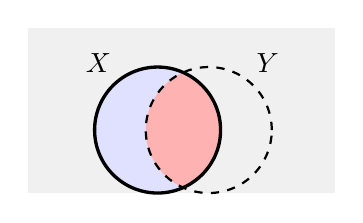
\begin{tikzpicture}[scale=0.5]
\fill[gray!12] (-3.3,-1.0) rectangle (4.5,3.2);
\begin{scope}
\clip (0,0.6) circle (1.6);
\fill[blue!12] (-3.3,-1.0) rectangle (4.5,3.2);
\fill[red!30] (1.3,0.6) circle (1.6);
\end{scope}
\draw[very thick] (0,0.6) circle (1.6);
\draw[thick,dashed] (1.3,0.6) circle (1.6);
\node at (-1.5,2.3) {\normalsize $X$};
\node at (2.8,2.3) {\normalsize $Y$};
\end{tikzpicture}

{\footnotesize \textbf{Conditional} $P(Y|X)$: zoom into just the $X$ circle (solid outline), ask what fraction of it is also $Y$ (dashed outline).}
\end{center}
\end{frame}

%%%%%%%%%%%%%%%%%%%%%%%%%%%%%%%%%%%%%%%%%%%%%%%%%%%%%%%%%%
\begin{frame}[fragile]\frametitle{Probability (recap): Dependent Variables}
\begin{itemize}
\item When $X$ and $Y$ are \emph{not} independent, the joint probability still factors, but through conditioning instead of a plain product: $P(X,Y) = P(Y|X) \times P(X)$.
\item Equally validly, it factors the other way round too: $P(X,Y) = P(X|Y) \times P(Y)$, same joint probability, just conditioned on the other variable. (Keep this in mind: equating these two is exactly how Bayes' Theorem is derived.)
\item Example: ice-cream sales are really affected by whether it's hot outside, so $P(\text{Sales}, \text{Hot}) = P(\text{Sales}|\text{Hot}) \times P(\text{Hot})$, not the independent-case product $P(\text{Sales})\times P(\text{Hot})$.
\end{itemize}
\end{frame}

%%%%%%%%%%%%%%%%%%%%%%%%%%%%%%%%%%%%%%%%%%%%%%%%%%%%%%%%%%
\begin{frame}[fragile]\frametitle{Probability (recap): Bayes Theorem Derivation}
Derivation: write the same joint probability both ways round (previous slide), then equate them.
\begin{align*}
P(X,Y) &= P(Y|X)\times P(X)\\
P(Y,X) &= P(X|Y)\times P(Y)\\
P(X,Y) &= P(Y,X) \qquad \text{(joint probability is symmetric)}\\
P(X,Y) &= P(Y|X)\times P(X) = P(X|Y)\times P(Y)
\end{align*}
\begin{block}{Bayes' Theorem}
\[
P(Y|X) = \frac{P(X|Y)\times P(Y)}{P(X)}
\]
\end{block}
\end{frame}

%%%%%%%%%%%%%%%%%%%%%%%%%%%%%%%%%%%%%%%%%%%%%%%%%%%%%%%%%%
\begin{frame}[fragile]\frametitle{Probability (recap): How to Read Bayes' Theorem}
\[
P(Y|X) = \frac{P(X|Y)\times P(Y)}{P(X)}
\]
\begin{itemize}
\item $P(Y|X)$ is the \textbf{posterior}: what we want, our updated belief about $Y$ after seeing evidence $X$.
\item $P(X|Y)$ is the \textbf{likelihood}: how probable the evidence $X$ is, if $Y$ were true.
\item $P(Y)$ is the \textbf{prior}: what we believed about $Y$ \emph{before} seeing any evidence at all.
\item $P(X)$ is the \textbf{evidence} (or normalizer): how probable the evidence is overall, regardless of $Y$.
\item In short: \emph{posterior} $\propto$ \emph{likelihood} $\times$ \emph{prior}. Read $\propto$ as ``is proportional to'': $P(X)$ is the same fixed number no matter which $Y$ we're testing, so it never changes which $Y$ comes out biggest, it only rescales the final answer.
\item That's why this shortcut is so common: skip computing $P(X)$ entirely, and just compare likelihood $\times$ prior across the candidate values of $Y$.
\end{itemize}
\end{frame}

%%%%%%%%%%%%%%%%%%%%%%%%%%%%%%%%%%%%%%%%%%%%%%%%%%%%%%%%%%
\begin{frame}[fragile]\frametitle{Example: Meeting Tom}
\begin{itemize}
\item On a college campus, you meet a guy, say ``Tom''. He appears Shy.
\item You are asked to guess whether Tom is a Math PhD student or a Business MBA student. Assume these are the only two types on that campus.
\item Your gut guess is probably: Math PhD student, since Math PhD students are stereotypically Shy.
\item Let's check if that gut guess is right, using Bayes' Theorem.
\end{itemize}
\begin{center}

\includegraphics[width=0.55\linewidth,keepaspectratio]{nb_maths_mba}
\end{center}
{\tiny (Ref: A visual guide to Bayesian thinking )}
\end{frame}

%%%%%%%%%%%%%%%%%%%%%%%%%%%%%%%%%%%%%%%%%%%%%%%%%%%%%%%%%%
\begin{frame}[fragile]\frametitle{Example: Prior and Likelihood Ratios}
\begin{itemize}
\item How many Math PhD students are there, compared to Business MBA students? Say 1:10. This is the \textbf{prior ratio}: the relative size of the two populations themselves, before we know anything about Tom.
\item Within Math PhD students, as many as 75\% are Shy.
\item Within Business MBA students, only about 15\% are Shy.
\item Those two percentages together form the \textbf{likelihood ratio}, 75:15.
\end{itemize}
\begin{center}
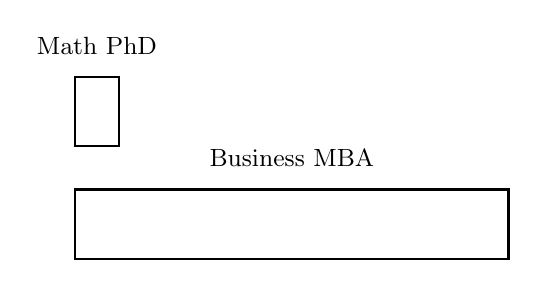
\begin{tikzpicture}[scale=0.55]
\draw[thick] (0,0) rectangle (10,1.6);
\node[above] at (5,1.9) {\small Business MBA};
\draw[thick] (0,2.6) rectangle (1,4.2);
\node[above] at (0.5,4.5) {\small Math PhD};
\end{tikzpicture}

{\footnotesize The two candidate populations, sized by the prior 1:10: Business MBA (wide) and Math PhD (narrow).}
\end{center}

{\tiny (Ref: A visual guide to Bayesian thinking )}
\end{frame}

%%%%%%%%%%%%%%%%%%%%%%%%%%%%%%%%%%%%%%%%%%%%%%%%%%%%%%%%%%
\begin{frame}[fragile]\frametitle{Example: Visualizing the Shaded Regions}
We need to find where Tom belongs. One thing is for sure: being Shy, he must be in one of those shaded patches. Let's compare just the shaded patches, side by side, at true scale:

\adjustbox{valign=t}{%
\begin{minipage}{0.45\linewidth}
\begin{center}

\includegraphics[width=0.85\linewidth,keepaspectratio]{nb_maths_mba}
\end{center}
\tiny{Original picture: both shaded patches together, at full context.}
\end{minipage}%
}%
\hfill%
\adjustbox{valign=t}{%
\begin{minipage}{0.5\linewidth}
\begin{center}
\begin{adjustbox}{max width=\linewidth}
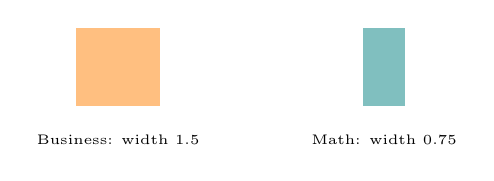
\begin{tikzpicture}[scale=0.7]
\filldraw[orange!50] (0,0) rectangle (1.5,1.4);
\node[below] at (0.75,-0.35) {\tiny Business: width 1.5};
\filldraw[teal!50] (5.2,0) rectangle (5.95,1.4);
\node[below] at (5.575,-0.35) {\tiny Math: width 0.75};
\end{tikzpicture}
\end{adjustbox}
\end{center}
\tiny{Just the two shaded patches, pulled out and compared at true scale.}
\end{minipage}%
}

{\small The Business Shy patch is twice as wide as the Math Shy patch, even though Math's Shy \emph{percentage} (75\%) is much higher than Business's (15\%). Higher percentage, but of a much smaller base.}

{\tiny (Ref: A visual guide to Bayesian thinking )}
\end{frame}

%%%%%%%%%%%%%%%%%%%%%%%%%%%%%%%%%%%%%%%%%%%%%%%%%%%%%%%%%%
\begin{frame}[fragile]\frametitle{Example: The Posterior Probability (Quick Method)}
A quick shortcut: multiply the prior ratio by the likelihood ratio, term by term:
\begin{center}
\begin{adjustbox}{max width=\linewidth}
$\underbrace{1}_{\text{Math prior}} \times \underbrace{75}_{\text{Math likelihood}} \; : \; \underbrace{10}_{\text{Business prior}} \times \underbrace{15}_{\text{Business likelihood}} \;=\; 75:150 \;=\; 1:2$
\end{adjustbox}
\end{center}
\begin{itemize}
\item That's the ratio of the two shaded areas from the previous slide, computed directly from the prior and likelihood ratios: no need to convert anything to actual probabilities first.
\item This combined ratio is called the \textbf{Posterior Probability} (ratio): our belief about Math vs.\ Business, updated after learning Tom is Shy.
\item Math : Business = 1 : 2, so Business MBA is now twice as likely as Math PhD.
\end{itemize}

{\tiny (Ref: A visual guide to Bayesian thinking )}
\end{frame}

%%%%%%%%%%%%%%%%%%%%%%%%%%%%%%%%%%%%%%%%%%%%%%%%%%%%%%%%%%
\begin{frame}[fragile]\frametitle{Example: The Posterior Probability (Full Bayes Substitution)}
Let's confirm this the long way, actually substituting into Bayes' Theorem. As fractions of the total population, the 1:10 prior means $P(\text{Math})=\tfrac{1}{11}$ and $P(\text{Business})=\tfrac{10}{11}$:
\begin{center}
\begin{adjustbox}{max width=\linewidth}
$\begin{aligned}
P(\text{Math}|\text{Shy}) &= \frac{P(\text{Shy}|\text{Math})\,P(\text{Math})}{P(\text{Shy})} = \frac{0.75 \times \frac{1}{11}}{P(\text{Shy})} \approx \frac{0.068}{P(\text{Shy})}\\
P(\text{Business}|\text{Shy}) &= \frac{P(\text{Shy}|\text{Business})\,P(\text{Business})}{P(\text{Shy})} = \frac{0.15 \times \frac{10}{11}}{P(\text{Shy})} \approx \frac{0.136}{P(\text{Shy})}
\end{aligned}$
\end{adjustbox}
\end{center}
\begin{itemize}
\item $P(\text{Shy})$ is the same shared denominator for both, so it can't change which one is bigger (the normalizer trick again), just compare numerators: $0.068 : 0.136 = 1:2$, exactly the quick method's answer.
\end{itemize}
\begin{center}
\begin{adjustbox}{max width=0.5\linewidth}
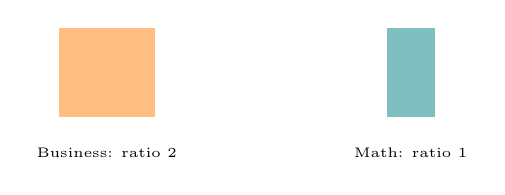
\begin{tikzpicture}[scale=0.8]
\filldraw[orange!50] (0,0) rectangle (1.5,1.4);
\node[below] at (0.75,-0.35) {\tiny Business: ratio 2};
\filldraw[teal!50] (5.2,0) rectangle (5.95,1.4);
\node[below] at (5.575,-0.35) {\tiny Math: ratio 1};
\end{tikzpicture}
\end{adjustbox}

{\small So, Tom is more likely to be a Business MBA student than a Math PhD student, despite the gut guess at the start!}
\end{center}

{\tiny (Ref: A visual guide to Bayesian thinking )}
\end{frame}

%%%%%%%%%%%%%%%%%%%%%%%%%%%%%%%%%%%%%%%%%%%%%%%%%%%%%%%%%%%%%%%%%%%%%%%%%%%%%%%%%%
\begin{frame}[fragile]\frametitle{}
\begin{center}
{\Large Bayes Learning}

{\tiny (Ref: Georgia tech, Udacity, Machine Learning)}

\end{center}


\end{frame}

%%%%%%%%%%%%%%%%%%%%%%%%%%%%%%%%%%%%%%%%%%%%%%%%%%%%%%%%%%
\begin{frame}[fragile]\frametitle{Bayesian Learning}
\begin{itemize}
\item Goal of machine learning is: We want best model/function for the given data.
\item Can we say? Its equivalent to: We want most ``probable'' model, for the given data.
\item That's represented by: $P(h|D)$ where h is hypothesis (think of it as a function) and D is data.
\item We can try many hypotheses, and find max of them.
\end{itemize}
\begin{center}
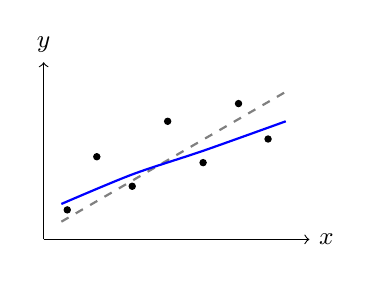
\begin{tikzpicture}[scale=0.75]
\draw[->] (0,0) -- (4.5,0) node[right] {\small $x$};
\draw[->] (0,0) -- (0,3) node[above] {\small $y$};
\foreach \p in {(0.4,0.5),(0.9,1.4),(1.5,0.9),(2.1,2.0),(2.7,1.3),(3.3,2.3),(3.8,1.7)}
\filldraw[black] \p circle (1.5pt);
\draw[thick,gray,dashed] (0.3,0.3) -- (4.1,2.5);
\draw[thick,blue] plot[smooth] coordinates {(0.3,0.6) (1.5,1.1) (2.7,1.5) (4.1,2.0)};
\end{tikzpicture}

{\small Many hypotheses (curves) could fit the data; the blue one is the most probable given $D$.}
\end{center}
\end{frame}

%%%%%%%%%%%%%%%%%%%%%%%%%%%%%%%%%%%%%%%%%%%%%%%%%%%%%%%%%%
\begin{frame}[fragile]\frametitle{Bayes Rule (recall)}

\begin{itemize}
\item We're about to reuse Bayes' Theorem, but now with $h$ (hypothesis) and $D$ (data) in place of $X$ and $Y$:
\end{itemize}
\[
P(h|D) = \frac{P(D|h)P(h)}{P(D)}
\]
\begin{itemize}
\item This is exactly the same formula from the previous slide, just relabeled: $h$ plays the role of $Y$, $D$ plays the role of $X$.
\item Chain Rule: $P(a \cap b) = P(a|b)P(b) = P(b|a)P(a)$, since $P(a\cap b)$ can be written either way round.
\end{itemize}

\begin{center}
\begin{adjustbox}{max width=0.4\linewidth}
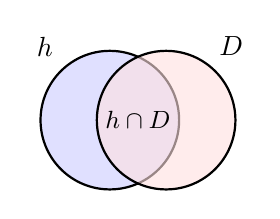
\begin{tikzpicture}[scale=0.55]
\draw[thick,fill=blue!12] (0,0.6) circle (1.6);
\draw[thick,fill=red!12,fill opacity=0.6] (1.3,0.6) circle (1.6);
\node at (-1.5,2.3) {\normalsize $h$};
\node at (2.8,2.3) {\normalsize $D$};
\node[align=center] at (0.65,0.6) {\small $h\cap D$};
\end{tikzpicture}
\end{adjustbox}

{\footnotesize The same picture as $P(Y|X)$ earlier: $h$ where $Y$ was, $D$ where $X$ was.}
\end{center}

\end{frame}

%%%%%%%%%%%%%%%%%%%%%%%%%%%%%%%%%%%%%%%%%%%%%%%%%%%
\begin{frame}[fragile]\frametitle{Bayes Rule: What Does Conditioning Mean?}
\begin{itemize}
\item $P(a|b)$ reads as ``probability of $a$, given $b$''.
\item Better way to understand it: restrict your attention to only the $b$ world (forget everything outside it), then ask how much of that restricted world is also $a$.
\item So $P(a|b)$ is $\dfrac{P(a \cap b)}{P(b)}$: the overlap, as a fraction of $b$ alone, not of everything.
\item This is why conditioning can shrink or grow a probability drastically: the denominator changes from ``everything'' to just ``$b$''.
\item This is exactly the same idea as $P(Y|X)$ from the Probability recap earlier: just relabeled $a,b$ instead of $Y,X$, the way this section relabels things to $h,D$.
\end{itemize}
\begin{center}
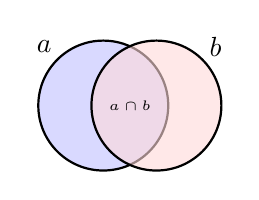
\begin{tikzpicture}[scale=0.75]
\draw[thick,fill=blue!15] (0,0.6) circle (1.1);
\draw[thick,fill=red!15,fill opacity=0.6] (0.9,0.6) circle (1.1);
\node at (-1.0,1.6) {$a$};
\node at (1.9,1.6) {$b$};
\node[align=center] at (0.45,0.6) {\tiny $a\cap b$};
\end{tikzpicture}

{\small $P(a|b)$: zoom into just the $b$ circle, ask what fraction of it overlaps $a$.}
\end{center}
\end{frame}

%%%%%%%%%%%%%%%%%%%%%%%%%%%%%%%%%%%%%%%%%%%%%%%%%%%%%%%%%%
\begin{frame}[fragile]\frametitle{De-constructing the formula}

\begin{center}
$P(h|D) = \dfrac{\overbrace{P(D|h)}^{\text{likelihood}}\;\overbrace{P(h)}^{\text{prior}}}{\underbrace{P(D)}_{\text{normalizer}}}$
\end{center}

\begin{itemize}
\item The bottom term, $P(D)$ is called as Prior on the Data, ie belief of seeing the data.
\item As we are comparing many hypotheses, and this bottom term being there in all such calculations, one can ignore it. It’s a normalization term.
\item $P(D|h)$ is like learning backwards. Its easy to see it in the machine learning dataset. Its basically the LIKELIHOOD of seeing Data given the hypothesis.
\item Note : $D = \{(x_i, y_i)\}$
\item So it means, given $x_i$, and the hypothesis that we are testing, meaning the function, whats the likelihood of seeing $y_i$?

\end{itemize}

\end{frame}

%%%%%%%%%%%%%%%%%%%%%%%%%%%%%%%%%%%%%%%%%%%%%%%%%%%%%%%%%%
\begin{frame}[fragile]\frametitle{Example: A Simple Hypothesis}
\begin{itemize}
\item Hypothesis h = return true if $x > 10$
\item Data $x = 7$
\item Now the question is what is the probability of $y == True$.
\item Its 0.
\item What for False?
\item Its 1.
\end{itemize}
\begin{center}
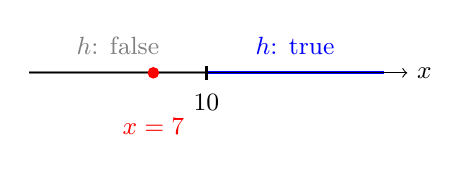
\begin{tikzpicture}[scale=0.75]
\draw[very thick,gray] (0,0) -- (3,0);
\draw[very thick,blue] (3,0) -- (6,0);
\draw[->] (0,0) -- (6.4,0) node[right] {\small $x$};
\draw[thick] (3,0.12) -- (3,-0.12);
\node[below] at (3,-0.2) {\small $10$};
\node[above,gray] at (1.5,0.15) {\small $h$: false};
\node[above,blue] at (4.5,0.15) {\small $h$: true};
\filldraw[red] (2.1,0) circle (2.5pt);
\node[below,red] at (2.1,-0.6) {\small $x=7$};
\end{tikzpicture}

{\small $x=7$ falls left of the threshold, squarely in ``false'' territory, hence $P(y{=}\text{True})=0$.}
\end{center}
\end{frame}

%%%%%%%%%%%%%%%%%%%%%%%%%%%%%%%%%%%%%%%%%%%%%%%%%%%%%%%%%%
\begin{frame}[fragile]\frametitle{Back to formula}

\begin{itemize}
\item As we have labeled data, its easier to compute/adjust $P(D|h)$ (as h and D are known) than $P(h|D)$
\item $P(h)$ is prior on $h$. 
\item Probability of this hypothesis $h$ occurring amongst all hypotheses. 
\item Its actually domain knowledge, the features, the type of model we are trying. 
\item It’s the probability of selected features or model.
\end{itemize}

\end{frame}



%%%%%%%%%%%%%%%%%%%%%%%%%%%%%%%%%%%%%%%%%%%%%%%%%%%%%%%%%%
\begin{frame}[fragile]\frametitle{Properties}

\begin{center}
$P(h|D)\ \textcolor{green!55!black}{\uparrow} \;=\; \dfrac{P(D|h)\,\textcolor{green!55!black}{\uparrow}\;\; P(h)\,\textcolor{green!55!black}{\uparrow}}{P(D)\ \text{(fixed)}}$
\end{center}

\begin{itemize}
\item If we have left hand side, ie ,$P(h|D)$ to go up, what should be changed on the right hand side?
\item $P(h)$ can go up. Probability of getting good hypothesis, ie better features or model, without seeing data, can go up
\item $P(D|h)$: Once you see data, for that data,  if you get that nicely predicting with $h$, then we are good. Good accuracy giving $h$.
\item $P(D)$ cannot change, (ie cannot go down)

\end{itemize}

\end{frame}

%%%%%%%%%%%%%%%%%%%%%%%%%%%%%%%%%%%%%%%%%%%%%%%%%%%%%%%%%%
\begin{frame}[fragile]\frametitle{Example: The Rare-Disease Test}

\begin{itemize}
\item A man goes to a doctor. He gives him a test for a rare disease. The test generally returns correct positive results 98% of times and correct negative results 97\% of times.
\item $TP=0.98, TN=0.97, FP=0.03, FN=0.02$
\item The disease in general, in the population is to only .8\% people.
\item The result: the test comes positive.
\item Question: Does he really have the disease?


\end{itemize}

\end{frame}

%%%%%%%%%%%%%%%%%%%%%%%%%%%%%%%%%%%%%%%%%%%%%%%%%%%%%%%%%%
\begin{frame}[fragile]\frametitle{Example: Applying Bayes Rule to the Test}

\begin{itemize}
\item We are looking for intersection set of $test=positive$ and $disease = true$
\end{itemize}

\begin{center}
\begin{adjustbox}{max width=0.42\linewidth}
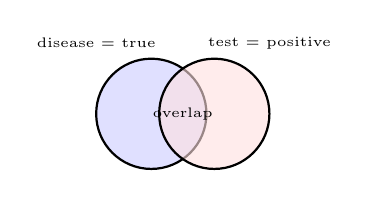
\begin{tikzpicture}[scale=0.5]
\draw[thick,fill=blue!12] (0,0.6) circle (1.4);
\draw[thick,fill=red!12,fill opacity=0.6] (1.6,0.6) circle (1.4);
\node at (-1.4,2.4) {\tiny disease $=$ true};
\node at (3.0,2.4) {\tiny test $=$ positive};
\node[align=center] at (0.8,0.6) {\tiny overlap};
\end{tikzpicture}
\end{adjustbox}
\end{center}

\begin{itemize}
\item Let’s apply Bayes rule to see probability of disease being there given the test has come out positive.
\item $P(disease=true|test=positive) = \frac{P(test=positive | disease=true)P(disease=true)}{P(test=positive)}$
\item Let’s see the probability of not having the disease even of the test said true
\item $P(disease=false|test=positive) = \frac{P(test=positive | disease=false)P(disease=false)}{P(test=positive)}$
\item Which is bigger?
\item As you can see, for comparison, the denominators are same, so we need not calculate it.

\end{itemize}

\end{frame}


%%%%%%%%%%%%%%%%%%%%%%%%%%%%%%%%%%%%%%%%%%%%%%%%%%%%%%%%%%
\begin{frame}[fragile]\frametitle{Solution}
Substituting numbers into the previous slide's formula: $P(\text{disease}|\text{positive}) = \dfrac{P(\text{positive}|\text{disease})\,P(\text{disease})}{P(\text{positive})}$, and skipping the shared denominator since we only need to compare the two:
\begin{itemize}
\item $P(disease=true|test=positive) \propto 0.98 \times 0.008 = 0.00784$
\item $P(disease=false|test=positive) \propto 0.03\times 0.992 = 0.02976$. This is bigger.
\item SO, don’t Panic!!
\item \textbf{Bottom line:} normalize just those two numbers.
  \begin{itemize}
  \item[] $P(\text{no disease}) = 0.02976/(0.02976+0.00784) \approx 0.79$
  \item[] About 79\% chance you're disease-free, even with a positive test. Only 21\% chance you actually have it.
  \end{itemize}
\end{itemize}

\begin{center}
\begin{adjustbox}{max width=0.6\linewidth}
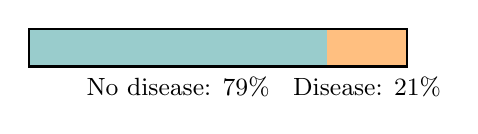
\begin{tikzpicture}[scale=0.6]
\filldraw[teal!40] (0,0) rectangle (6.32,0.8);
\filldraw[orange!50] (6.32,0) rectangle (8,0.8);
\draw[thick] (0,0) rectangle (8,0.8);
\node[below] at (3.16,0) {\small No disease: 79\%};
\node[below] at (7.16,0) {\small Disease: 21\%};
\end{tikzpicture}
\end{adjustbox}
\end{center}

\end{frame}

%%%%%%%%%%%%%%%%%%%%%%%%%%%%%%%%%%%%%%%%%%%%%%%%%%%%%%%%%%
\begin{frame}[fragile]\frametitle{Algorithm}



\begin{itemize}
\item Good part is, as we want argmax only, we don’t need denominator P(D) , which is hard to calculate anyway.
\item $P(h)$ is also hard to compute. So if we further drop that and find $argmax P(D|h)$ than its called Maximum Likelihood Hypothesis. 
\item That just makes an assumption, that all $P(h)$ are same. 
\item All model or feature scheme are equally likely
\end{itemize}

\begin{lstlisting}
For each h in H
    Calculate p(h|D) = P(D|h)P(h)/P(D)
Output:
    H = argmax_h P(h|D)

\end{lstlisting}

\end{frame}

%%%%%%%%%%%%%%%%%%%%%%%%%%%%%%%%%%%%%%%%%%%%%%%%%%%%%%%%%%%%%%%%%%%%%%%%%%%%%%%%%%
\begin{frame}[fragile]\frametitle{}
\begin{center}
{\Large Bayesian Classifier}
\end{center}

\end{frame}

%%%%%%%%%%%%%%%%%%%%%%%%%%%%%%%%%%%%%%%%%%%%%%%%%%%%%%%%%%
\begin{frame}[fragile]\frametitle{Connecting the Dots}
\begin{itemize}
\item The rare-disease example we just worked through \emph{was} a classifier: given a test result, decide between two classes, ``has disease'' and ``no disease''.
\item We used $P(h|D)$ for a hypothesis $h$; a classifier instead asks $P(y|x)$ for a class label $y$ given features $x$, exactly the same idea, just renamed for the classification setting.
\item The next few slides make this formal: a general recipe for turning Bayes' Theorem into a working classifier.
\end{itemize}
\end{frame}


%%%%%%%%%%%%%%%%%%%%%%%%%%%%%%%%%%%%%%%%%%%%%%%%%%%%%%%%%%
\begin{frame}[fragile]\frametitle{Bayes Classifier: What Is It?}
%\begin{center}
%
\includegraphics[width=0.6\linewidth,keepaspectratio]{nb1}
%\end{center}
	\begin{itemize}
	\item A classifier is a function
	\item It takes features as inputs, so $x_1,x_2 \ldots$
	\item Gives y as output, which could be $y=1,y=2,\ldots$. These are the classes. For binary classifier y can take only $0,1$.
	\item x can be real or numeric and it could also be categorical.
	\item With training data, the function is learnt. That's the classifier model.
	\end{itemize}

\end{frame}

%%%%%%%%%%%%%%%%%%%%%%%%%%%%%%%%%%%%%%%%%%%%%%%%%%%%%%%%%%
\begin{frame}[fragile]\frametitle{Bayes Classifier: Picking the Max Probability}
%\begin{center}
%
\includegraphics[width=0.6\linewidth,keepaspectratio]{nb1}
%\end{center}
	\begin{itemize}
	\item Bayesian Classifier is probabilistic.
	\item Meaning, it does not produce y class values directly,  but it gives probabilities of $y=0$ and $y=1$
	\item We pick max and say that, that's the output class
	\item $\hat{y} = arg max P (y|x)$
	\end{itemize}

\end{frame}


%%%%%%%%%%%%%%%%%%%%%%%%%%%%%%%%%%%%%%%%%%%%%%%%%%%%%%%%%%%
%\begin{frame}[fragile]\frametitle{Bayesian classification }
%Bayes Theorem: $P(Y|X) = \frac{P(X|Y)(P(Y)}{P(X)}$
%\begin{itemize}
%\item P(Y|X) : Probability that the customer will buy a computer given that 
%we know his age, credit rating and income. (Posterior Probability of Y)
%\item P(Y) : Probability that the customer will buy a computer regardless 
%of age, credit rating, income (Prior Probability of Y)
%\item P(X|Y) : Probability that the customer is 35 yrs old, have fair credit 
%rating and earns \$40,000, given that he has bought our computer 
%(Posterior Probability of X)
%\item P(X) : Probability that a person from our set of customers is 35 yrs 
%old, have fair credit rating and earns \$40,000. (Prior Probability of X). 
%\end{itemize}
%\end{frame}


% Cut (deck-review pass): the "buy a computer" example lasted only these 2 frames and never
% paid off with a numeric result. nb4's X/Y-as-dataset framing duplicates "Bayes Classifier:
% What Is It?" two frames earlier, and nb3's denominator-expansion lesson is fully retaught,
% with actual numbers, by the Ebola "...: The Evidence P(x)" frame below. Left commented, not
% deleted, in case the nb3/nb4 images are wanted elsewhere.
% %%%%%%%%%%%%%%%%%%%%%%%%%%%%%%%%%%%%%%%%%%%%%%%%%%%%%%%%%%
% \begin{frame}[fragile]\frametitle{Bayesian Classification: A Worked Setup}
% Example
% \begin{center}
% 
\includegraphics[width=0.6\linewidth,keepaspectratio]{nb4}
% \end{center}
% \begin{itemize}
% \item X: Independent Variables: Age, Income, Credit Rating
% \item Y: Dependent Variable: Will buy computer or not? Binary.
% \end{itemize}
% \end{frame}
%
% %%%%%%%%%%%%%%%%%%%%%%%%%%%%%%%%%%%%%%%%%%%%%%%%%%%%%%%%%%
% \begin{frame}[fragile]\frametitle{Bayesian Classification: Expanding the Denominator}
% Bayesian probability of a class:
% \begin{center}
% 
\includegraphics[width=0.6\linewidth,keepaspectratio]{nb3}
% \end{center}
% \begin{itemize}
% \item Where denominator term of Bayes Theorem: $P(Y|X) = \frac{P(X|Y)P(Y)}{P(X)}$ is expanded
% \item Its summation of Probabilities that customer is 35 given that he buys computer, customer has fair credit rating given that he buys computer, and so on. And, also similarly for when he does not buy computer.
% \end{itemize}
% \end{frame}

% Moved earlier (deck-review pass, 2026-09-11): these two frames used to sit right after the
% Spam/Laplace worked example, explaining the independence trick only after it had already been
% used silently -- moved here, right after the classifier's argmax definition and before any
% example uses the trick, so the Spam example below can lean on it explicitly instead of
% assuming it.
%%%%%%%%%%%%%%%%%%%%%%%%%%%%%%%%%%%%%%%%%%%%%%%%%%%%%%%%%%
\begin{frame}[fragile]\frametitle{Independence Assumption: The Trick}
\begin{itemize}
\item Trick is to assume that all these x variables are independent, given y.
\item That makes combined probability as just multiplication of individual conditional probabilities.
\item So, it becomes sum of multiplications only
\begin{center}
% 
\includegraphics[width=\linewidth,keepaspectratio]{nb1} -- too fuzzy at slide size; formula transcribed below instead.
\begin{adjustbox}{max width=\linewidth}
$\displaystyle P(x_1\ldots x_d|y) = \underbrace{\prod_{i=1}^{d} P(x_i|x_1\ldots x_{i-1},y)}_{\text{chain rule (exact)}} = \underbrace{\prod_{i=1}^{d} P(x_i|y)}_{\text{independence}}$
\end{adjustbox}
\end{center}
\item Individual probabilities are: e.g. whats probability of a particular word appearing, given the message is spam.
\item Multiply for all variables $x_i$'s: this is exactly the trick the Spam example below relies on.
\end{itemize}
\end{frame}

%%%%%%%%%%%%%%%%%%%%%%%%%%%%%%%%%%%%%%%%%%%%%%%%%%%%%%%%%%
\begin{frame}[fragile]\frametitle{Independence Assumption: The Chain Rule}
\begin{itemize}
\item Joint probability of $y$ and many features $x_1,x_2,x_3,\ldots,x_n$ can be expressed as the chain rule:

$P(y,x_1,x_2,x_3,\ldots,x_n)$

$= P(x_1,x_2,x_3,\ldots,x_n|y)P(y)$

$= P(y)P(x_1|y)P(x_2|y,x_1)P(x_3|y,x_1,x_2)\ldots$

\item This is messy, but if we naively assume independence, then

$P(x_2|y,x_1) = P(x_2|y)$

$P(x_3|y,x_1,x_2) = P(x_3|y)$

$P(x_n|y,x_1,x_2,\ldots) = P(x_n|y)$

\end{itemize}

\begin{block}{Intuition}
Without this assumption, estimating the joint probability of many features would need a
training example for nearly every possible combination of feature values, practically
impossible once you have more than a handful of features. Assuming conditional independence
collapses that into one small probability per feature, each estimated separately from the
data, which is why the ``naive'' shortcut is what makes the classifier usable at all.
\end{block}
\end{frame}

% Replaced (deck-review pass): the Ebola example (4 frames) was purely conceptual, never
% worked a single number, and largely duplicated the Rare-Disease-Test example already covered.
% Swapped for the classic spam/ham example instead -- the single most famous real-world Naive
% Bayes application (Paul Graham's "A Plan for Spam"), which also gives the deck its first
% text/word-features example and a natural, honest reason to need Laplace smoothing.
%%%%%%%%%%%%%%%%%%%%%%%%%%%%%%%%%%%%%%%%%%%%%%%%%%%%%%%%%%
\begin{frame}[fragile]\frametitle{Example: The Spam Dataset}
A tiny training set of 8 messages, labeled by a human as Normal or Spam:
\begin{center}
\small
\begin{tabular}{cl|cl}
\multicolumn{2}{c|}{\textbf{Normal}} & \multicolumn{2}{c}{\textbf{Spam}} \\ \hline
N1 & meeting today at noon    & S1 & win money now \\
N2 & please send the report   & S2 & click here to win \\
N3 & lunch with the team      & S3 & free money offer \\
N4 & thanks for the help      & S4 & win a free gift
\end{tabular}
\end{center}
\begin{itemize}
\item Class $y \in \{\text{normal}, \text{spam}\}$.
\item Features $x_1, x_2, \ldots$: one feature per word, each a yes/no flag for ``does this word appear in the message'' (1 or 0).
  \begin{itemize}
  \item Example: $x_{\text{win}}=1$ if the message contains the word ``win'', else $0$. Likewise $x_{\text{free}}$, $x_{\text{money}}$, and so on for every word we track.
  \item A message is turned into a long list of these 1/0 flags, one per word in our vocabulary: that list is $x$.
  \end{itemize}
\item Goal: given a new message's word-flags $x$, decide $\hat{y} = \arg\max_y P(y|x)$, the same $\arg\max$ recipe from the classifier definition.
\end{itemize}
\end{frame}

%%%%%%%%%%%%%%%%%%%%%%%%%%%%%%%%%%%%%%%%%%%%%%%%%%%%%%%%%%
\begin{frame}[fragile]\frametitle{Example: Word Counts by Class}
\begin{itemize}
\item Priors, straight from the message counts: $P(\text{normal}) = 4/8 = 0.5$, $P(\text{spam}) = 4/8 = 0.5$.
\item For three words we'll need next: ``win'' appears in 0 of 4 Normal messages but 3 of 4 Spam messages; ``money'' in 0 of 4 Normal but 2 of 4 Spam; ``free'' in 0 of 4 Normal but 2 of 4 Spam.
\end{itemize}
\begin{center}
\begin{adjustbox}{max width=\linewidth}
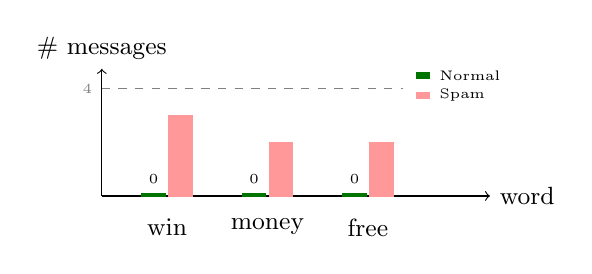
\begin{tikzpicture}[scale=0.85]
\draw[->] (0,0) -- (5.8,0) node[right] {\small word};
\draw[->] (0,0) -- (0,1.9) node[above] {\small \# messages};
\draw[dashed,gray] (0,1.6) -- (4.5,1.6);
\node[left,gray] at (0,1.6) {\tiny 4};
% win
\filldraw[green!45!black] (0.6,0) rectangle (0.95,0.04);
\node[above] at (0.775,0.04) {\tiny 0};
\filldraw[red!40] (1.0,0) rectangle (1.35,1.2);
\node[below] at (0.975,-0.2) {\small win};
% money
\filldraw[green!45!black] (2.1,0) rectangle (2.45,0.04);
\node[above] at (2.275,0.04) {\tiny 0};
\filldraw[red!40] (2.5,0) rectangle (2.85,0.8);
\node[below] at (2.475,-0.2) {\small money};
% free
\filldraw[green!45!black] (3.6,0) rectangle (3.95,0.04);
\node[above] at (3.775,0.04) {\tiny 0};
\filldraw[red!40] (4.0,0) rectangle (4.35,0.8);
\node[below] at (3.975,-0.2) {\small free};
% legend
\filldraw[green!45!black] (4.7,1.75) rectangle (4.9,1.85);
\node[right] at (4.9,1.8) {\tiny Normal};
\filldraw[red!40] (4.7,1.45) rectangle (4.9,1.55);
\node[right] at (4.9,1.5) {\tiny Spam};
\end{tikzpicture}
\end{adjustbox}

{\tiny Paired bars per word: green is the count among Normal messages (out of 4), red is the count among Spam messages (out of 4). Every green bar is flush at 0: none of these three words show up in any Normal message.}
\end{center}
\end{frame}

%%%%%%%%%%%%%%%%%%%%%%%%%%%%%%%%%%%%%%%%%%%%%%%%%%%%%%%%%%
\begin{frame}[fragile]\frametitle{Example: Likelihoods for a New Message}
New message to classify: \emph{``win free money''}.
\begin{center}
\begin{tabular}{l|c|c}
\textbf{Word} & \textbf{$P(\text{word}|\text{normal})$} & \textbf{$P(\text{word}|\text{spam})$} \\ \hline
win   & $0/4 = 0$ & $3/4 = 0.75$ \\
free  & $0/4 = 0$ & $2/4 = 0.5$ \\
money & $0/4 = 0$ & $2/4 = 0.5$
\end{tabular}
\end{center}
\begin{itemize}
\item Naive Bayes recipe: $P(y|\text{msg}) \propto P(y) \times \prod_{\text{word}} P(\text{word}|y)$, multiply the prior by every word's likelihood. This product is exactly the independence trick from before, applied to these three words.
\item For \textbf{Normal}: $P(\text{normal})\times P(\text{win}|\text{normal})\times P(\text{free}|\text{normal})\times P(\text{money}|\text{normal}) = 0.5\times0\times0\times0=0$.
\item \textbf{Yikes}: multiplying by even a single $0$ wipes out the whole product, no matter what the other factors are. None of these three words ever showed up in our (tiny) set of Normal messages, so the model declares this message \emph{impossible} to be Normal, not just unlikely.
\item That's too strong a claim from just 4 examples: a bigger inbox would eventually show ``money'' in an ordinary message too (a bill, a salary email).
\end{itemize}
\end{frame}

%%%%%%%%%%%%%%%%%%%%%%%%%%%%%%%%%%%%%%%%%%%%%%%%%%%%%%%%%%
\begin{frame}[fragile]\frametitle{Laplace (Add-One) Smoothing}
\[
P(x_i|y_j) = \frac{n_c + 1}{n + k}
\]
\begin{itemize}
\item $n$ = number of training messages of class $y_j$ (here, 4 for either class).
\item $n_c$ = number of those messages that contain the word $x_i$.
\item $k$ = number of values the feature can take: here $k=2$ for every word (present or absent). Adding $k$ (not just $1$) to the denominator keeps $P(\text{present}|y_j)+P(\text{absent}|y_j)=1$ even after the pretend extra messages below are added in.
\item This directly fixes the ``Yikes'' problem from before: $P(\text{win}|\text{normal})$ becomes $\dfrac{0+1}{4+2}=\dfrac{1}{6}\approx0.167$ instead of a hard, message-killing $0$.
\end{itemize}
\begin{block}{Intuition}
Pretend we've already seen one extra, evenly-spread-out message for every class: one where the
word is present, one where it's absent. A count that was genuinely 0 becomes a small positive
number instead of a hard impossibility; counts that were already large barely change.
\end{block}
\end{frame}

%%%%%%%%%%%%%%%%%%%%%%%%%%%%%%%%%%%%%%%%%%%%%%%%%%%%%%%%%%
\begin{frame}[fragile]\frametitle{Example: Smoothed Likelihoods and the Final Call}
With $n=4$, $k=2$:
\begin{center}
\begin{tabular}{l|c|c}
\textbf{Word} & \textbf{$P(\text{word}|\text{normal})$} & \textbf{$P(\text{word}|\text{spam})$} \\ \hline
win   & $\frac{0+1}{4+2}=\frac{1}{6}\approx0.167$ & $\frac{3+1}{4+2}=\frac{4}{6}\approx0.667$ \\
free  & $\frac{0+1}{4+2}=\frac{1}{6}\approx0.167$ & $\frac{2+1}{4+2}=\frac{3}{6}=0.5$ \\
money & $\frac{0+1}{4+2}=\frac{1}{6}\approx0.167$ & $\frac{2+1}{4+2}=\frac{3}{6}=0.5$
\end{tabular}
\end{center}
\begin{align*}
P(\text{normal}|\text{msg}) &\propto 0.167\times0.167\times0.167\times0.5 \approx 0.0023 \\
P(\text{spam}|\text{msg})   &\propto 0.667\times0.5\times0.5\times0.5 \approx 0.0834
\end{align*}
\begin{itemize}
\item We skip the shared denominator $P(\text{evidence})$: it's the same constant for both classes, so it can't change which one is bigger, the normalizer trick from before.
\item $0.0834 \gg 0.0023$: classified as \textbf{Spam}, by roughly the same margin the raw (unsmoothed) numbers already suggested, just without the false certainty of an outright zero.
\item Concretely, $0.0834/0.0023 \approx 36$: Spam is roughly \textbf{36 times} more likely than Normal for this message, a confident call, not a coin flip.
\end{itemize}
\end{frame}

%
%
%%%%%%%%%%%%%%%%%%%%%%%%%%%%%%%%%%%%%%%%%%%%%%%%%%%%%%%%%%%
%\begin{frame}[fragile]\frametitle{Normalization Example}
%
%\begin{center}
%
\includegraphics[width=0.6\linewidth,keepaspectratio]{nb2}
%\end{center}
%
%\begin{itemize}
%\item Its a digit recognition program. 
%\item Output class y is ether 3 or 6.
%\item Features are x1 and x2, say, x1 represent amount of ink.
%\end{itemize}
%
%\end{frame}
%
%
%%%%%%%%%%%%%%%%%%%%%%%%%%%%%%%%%%%%%%%%%%%%%%%%%%%%%%%%%%%
%\begin{frame}[fragile]\frametitle{Normalization Example}
%
%\begin{center}
%
\includegraphics[width=0.6\linewidth,keepaspectratio]{nb2}
%\end{center}
%
%\begin{itemize}
%\item Look at outlier marked with x1.
%\item Its has so much ink (ie x1) so it does not know how to classify.
%\item So probability of this being classified as any class , 3 or 6, very very low.
%\item So x2 has more probability compare to x1, given that its a 3.
%
%\end{itemize}
%
%\end{frame}
%
%
%%%%%%%%%%%%%%%%%%%%%%%%%%%%%%%%%%%%%%%%%%%%%%%%%%%%%%%%%%%
%\begin{frame}[fragile]\frametitle{Normalization}
%\begin{itemize}
%\item What does Normalizer $P(x) = \sum P(x|y')P(y')$ do?
%\item It affects outlier. 
%\item Outlier has a low probability under every class.
%\item This being in denominator, boost the overall outcome of $P(Y=3|X=x_1)$ and sort of normalizes the outliers like any other
%\end{itemize}
%\begin{center}
%
\includegraphics[width=0.6\linewidth,keepaspectratio]{nb2}
%\end{center}
%\end{frame}
%

% %%%%%%%%%%%%%%%%%%%%%%%%%%%%%%%%%%%%%%%%%%%%%%%%%%%%%%%%%%
% \begin{frame}[fragile]\frametitle{Independence assumption }
% \begin{itemize}
% \item When we need to compute $P(x|y)$, the x is actually many features.
% \item For Bitmaps 20x20, there are 400 x variables
% \item So there are $2^{400}$ patterns of x, 
% \item Probability of all these patterns is needed in deciding y=3 or y=6.
% \item That's too much!!
% \end{itemize}
% \end{frame}

%%%%%%%%%%%%%%%%%%%%%%%%%%%%%%%%%%%%%%%%%%%%%%%%%%%%%%%%%%%
%\begin{frame}[fragile]\frametitle{Independence assumption }
%\begin{itemize}
%\item Compute $P(x_1 \ldots x_n | y)$ for every observation $x_1 \ldots x_n$
%	\begin{itemize}
%	\item class-conditional ``counts'', based on training data
%	\item problem: may not have seen every $x_1 \ldots x_n$ for every $y$
%	\end{itemize}
%\item Probabilistic classification: most probable class given observation: $\hat{y} = arg~max_y P(y|x)$
%\item Idea: Assume $x_1 \ldots x_n$ conditionally independent given $y$
%\item So, it becomes sum of multiplications only
%\begin{center}
%
\includegraphics[width=\linewidth,keepaspectratio]{nb1}
%\end{center}
%\end{itemize}
%\end{frame}


%%%%%%%%%%%%%%%%%%%%%%%%%%%%%%%%%%%%%%%%%%%%%%%%%%%%%%%%%
\begin{frame}[fragile]\frametitle{Why is Bayes Classifier so popular?}
\begin{itemize}
\item Look at what it eventually comes down to. 
\item Just some counting and multiplication.
\item We can pre-compute all these terms, and so classifying becomes easy, quick and efficient. 
\end{itemize}
\end{frame}


%%%%%%%%%%%%%%%%%%%%%%%%%%%%%%%%%%%%%%%%%%%%%%%%%%%%%%%%%%%%%%%%%%%%%%%%%%%%%%%%%%
\begin{frame}[fragile]\frametitle{}
\begin{center}
{\Large Naive Bayes Example - Fruits Classification}
\end{center}
\end{frame}

%%%%%%%%%%%%%%%%%%%%%%%%%%%%%%%%%%%%%%%%%%%%%%%%%%%%%%%%%%
\begin{frame}[fragile]\frametitle{Example: The Fruit Dataset}
\begin{itemize}
\item So, let's say we have data on 1000 pieces of fruit. 
\item we know 3 features of each fruit, whether it's long or not, sweet or not and yellow or not
\item Outcome is the type: a Banana, Orange or some Other fruit.
\end{itemize}
\end{frame}


%%%%%%%%%%%%%%%%%%%%%%%%%%%%%%%%%%%%%%%%%%%%%%%%%%%%%%%%%%
\begin{frame}[fragile]\frametitle{Example: Counting the Fruits}
% \begin{center}
% 
\includegraphics[width=0.6\linewidth,keepaspectratio]{nb8}
% \end{center}
\begin{center}
\begin{tabular}{l|c|c|c|c}
\textbf{Fruit} & \textbf{Long} & \textbf{Sweet} & \textbf{Yellow} & \textbf{Total} \\ \hline
Banana & 400 & 350 & 450 & 500 \\
Orange & 0 & 150 & 300 & 300 \\
Other & 100 & 150 & 50 & 200 \\ \hline
\textbf{Total} & \textbf{500} & \textbf{650} & \textbf{800} & \textbf{1000}
\end{tabular}
\end{center}
So from the table what do we already know?
\begin{itemize}
\item     50\% of the fruits are bananas
\item     30\% are oranges
\item     20\% are other fruits
\end{itemize}

\end{frame}

%%%%%%%%%%%%%%%%%%%%%%%%%%%%%%%%%%%%%%%%%%%%%%%%%%%%%%%%%%
\begin{frame}[fragile]\frametitle{Example: The Full Training Table}
More explicit table
% \begin{center}
% 
\includegraphics[width=\linewidth,keepaspectratio]{nb9}
% \end{center}
\begin{center}
\adjustbox{max width=\linewidth}{
\begin{tabular}{l|cc|cc|cc|c}
\textbf{Type} & \textbf{Long} & \textbf{Not Long} & \textbf{Sweet} & \textbf{Not Sweet} & \textbf{Yellow} & \textbf{Not Yellow} & \textbf{Total} \\ \hline
Banana & 400 & 100 & 350 & 150 & 450 & 50 & 500 \\
Orange & 0 & 300 & 150 & 150 & 300 & 0 & 300 \\
Other Fruit & 100 & 100 & 150 & 50 & 50 & 150 & 200 \\ \hline
\textbf{Total} & \textbf{500} & \textbf{500} & \textbf{650} & \textbf{350} & \textbf{800} & \textbf{200} & \textbf{1000}
\end{tabular}
}
\end{center}
This is our 'training set.' We will use this to predict the type of any new fruit we encounter.
\end{frame}

%%%%%%%%%%%%%%%%%%%%%%%%%%%%%%%%%%%%%%%%%%%%%%%%%%%%%%%%%%
\begin{frame}[fragile]\frametitle{Example: The Fruit Priors}
We can pre-compute a lot of things about our fruit collection.
\begin{itemize}
\item     The so-called ``Prior'' probabilities. 
\item If we didn't know any of the fruit attributes, this would be our guess.
\item These are our base rates. $P(y)$.
\item P(Banana)      = 0.5 (500/1000)
\item  P(Orange)      = 0.3
\item  P(Other Fruit) = 0.2
\end{itemize}
\end{frame}

%%%%%%%%%%%%%%%%%%%%%%%%%%%%%%%%%%%%%%%%%%%%%%%%%%%%%%%%%%
\begin{frame}[fragile]\frametitle{Example: The Fruit Evidence P(x)}
Probability of ``Evidence''. $P(x)$
\begin{itemize}
\item P(Long)   = 0.5
\item P(Sweet)  = 0.65
\item P(Yellow) = 0.8
\end{itemize}
\end{frame}


%%%%%%%%%%%%%%%%%%%%%%%%%%%%%%%%%%%%%%%%%%%%%%%%%%%%%%%%%%
\begin{frame}[fragile]\frametitle{Example: Likelihoods for Banana}
Based on our training set we can also say the following:
\begin{itemize}
\item From 500 bananas 400 (0.8) are Long, So $P(Long|Banana) = 0.8$
\item 350 (0.7) are Sweet. So, $P(Sweet|Banana) = 0.7$
\item 450 (0.9) are Yellow, So, $P(Yellow|Banana) = 0.9$
\end{itemize}
\end{frame}

%%%%%%%%%%%%%%%%%%%%%%%%%%%%%%%%%%%%%%%%%%%%%%%%%%%%%%%%%%
\begin{frame}[fragile]\frametitle{Example: Likelihoods for Orange}
\begin{itemize}
\item Out of 300 oranges 0 are Long. So, $P(Long|Orange) = 0$. [Oranges are never long in all the fruit we have seen.]
\item 150 (0.5) are Sweet . So, $P(Sweet|Orange) = 0.5$
\item 300 (1) are Yellow.  So, $P(Yellow|Orange) = 1$
\end{itemize}
\end{frame}


%%%%%%%%%%%%%%%%%%%%%%%%%%%%%%%%%%%%%%%%%%%%%%%%%%%%%%%%%%
\begin{frame}[fragile]\frametitle{Example: Likelihoods for Other Fruit}
\begin{itemize}
\item From the remaining 200 fruits, 100 (0.5) are Long,  So $P(Long|Other) = 0.5$
\item 150 (0.75) are Sweet.  So $P(Sweet|Other) = 0.75$
\item 50 (0.25) are Yellow.  So $P(Yellow|Other) = 0.25$
\item Similarly, $P(Not Yellow|Other) = 0.75$ and so on
\end{itemize}
\end{frame}




%%%%%%%%%%%%%%%%%%%%%%%%%%%%%%%%%%%%%%%%%%%%%%%%%%%%%%%%%%
\begin{frame}[fragile]\frametitle{Example: Classifying a New Fruit}
Testing
\begin{itemize}
\item Given the features of a piece of fruit and we need to predict the class
\item Test fruit is Long, Sweet and Yellow
\item The one (fruit) with the highest probability (score) being the winner.
\end{itemize}

\end{frame}

%%%%%%%%%%%%%%%%%%%%%%%%%%%%%%%%%%%%%%%%%%%%%%%%%%%%%%%%%%
\begin{frame}[fragile]\frametitle{Example: The Fruit Classification Result}
% \begin{center}
% 
\includegraphics[width=\linewidth,keepaspectratio]{nb10}
% \end{center}
\small
\begin{align*}
P(\text{Banana}|L,S,Y) &= \frac{P(L|\text{Ba})\times P(S|\text{Ba})\times P(Y|\text{Ba})\times P(\text{Ba})}{P(\text{evidence})}\\
&= \frac{0.8\times0.7\times0.9\times0.5}{P(\text{evidence})} = \frac{0.252}{P(\text{evidence})}
\end{align*}
\[
P(\text{Orange}|L,S,Y) = 0 \qquad \text{(since } P(L|\text{Orange})=0\text{)}
\]
\begin{align*}
P(\text{Other}|L,S,Y) &= \frac{(100/200)\times(150/200)\times(50/200)\times(200/1000)}{P(\text{evidence})}\\
&= \frac{0.01875}{P(\text{evidence})}
\end{align*}
\normalsize
\begin{itemize}
\item $L$=Long, $S$=Sweet, $Y$=Yellow, Ba=Banana.
\end{itemize}
By an overwhelming margin $(0.252 \gg 0.01875)$, we classify this Sweet/Long/Yellow fruit as likely to be a Banana.
 \end{frame}


%%%%%%%%%%%%%%%%%%%%%%%%%%%%%%%%%%%%%%%%%%%%%%%%%%%%%%%%%%
%\begin{frame}[fragile]\frametitle{Predicted Probability Example}
%Scenario:
%
%\begin{itemize}
%\item A doctor knows that meningitis causes a stiff neck 50\% of the time
%\item Prior probability of any patient having meningitis is 1/50,000
%\item Prior probability of any patient having a stiff neck is 1/20
%\item If a patient has a stiff neck, what's the probability that they have meningitis?
%\item Apply Bayes' Rule:
%\begin{center}
%
\includegraphics[width=0.5\linewidth,keepaspectratio]{nbneck}
%\end{center}
%\end{itemize}
%Very low probability
%
%\end{frame}

% Cut for deck-size reduction (Aug 2026): the loan-default block (intro, Estimating Priors,
% and the Laplace smoothing follow-up) duplicated the fruit example's teaching purpose with a
% second full dataset. Left commented rather than deleted in case it's wanted back.
% Update (deck-review pass): the zero-probability "Yikes" moment and its Laplace-smoothing
% resolution are now taught via the Spam example above instead (reusing this section's own
% formula and Intuition block almost verbatim, with spam/word numbers in place of loan/Refund
% ones), so this loan-default version is now purely redundant/archival, not a missing piece.
% %%%%%%%%%%%%%%%%%%%%%%%%%%%%%%%%%%%%%%%%%%%%%%%%%%%%%%%%%%%%%%%%%%%%%%%%%%%%%%%%%%
% \begin{frame}[fragile]\frametitle{}
% \begin{center}
% {\Large Naive Bayes Example - Loan Default}
% \end{center}
% \end{frame}
% 
% %%%%%%%%%%%%%%%%%%%%%%%%%%%%%%%%%%%%%%%%%%%%%%%%%%%%%%%%%%
% \begin{frame}[fragile]\frametitle{Example: The Loan Default Problem}
% \adjustbox{valign=t}{
% \begin{minipage}{0.45\linewidth}
% 
% \begin{center}
% 
\includegraphics[width=\linewidth,keepaspectratio]{nbnecktble}
% \end{center}
% 
% \end{minipage}
% }
% \hfill
% \adjustbox{valign=t}{
% \begin{minipage}{0.45\linewidth}
% 
% \begin{itemize}
% \item Target class: Evade (this is our earlier loan-default table, revisited)
% \item Predictor variables: Refund, Status, Income
% \item What is probability of Evade given the values of Refund, Status, Income?
% \item $P(E|R,S,I)$
% %\item Above .5? Predict YES, else predict NO.
% \end{itemize}
% 
% \end{minipage}
% }
% \end{frame}
% 
% 
% %%%%%%%%%%%%%%%%%%%%%%%%%%%%%%%%%%%%%%%%%%%%%%%%%%%%%%%%%%
% \begin{frame}[fragile]\frametitle{Example: A New Test Instance}
% \adjustbox{valign=t}{
% \begin{minipage}{0.45\linewidth}
% 
% \begin{center}
% 
\includegraphics[width=\linewidth,keepaspectratio]{nbnecktble}
% \end{center}
% 
% \end{minipage}
% }
% \hfill
% \adjustbox{valign=t}{
% \begin{minipage}{0.45\linewidth}
% 
% \begin{itemize}
% \item Test instance is (same table as before):
% \begin{itemize}
% \item Refund=Yes
% \item Status=Married
% \item Income=60K
% \end{itemize}
% \item Issue: we don't have any training example that these same three attributes values.
% \item How to compute? $P(E|R,S,I)$
% %\item What are values of R, S, I?
% 
% \end{itemize}
% 
% \end{minipage}
% }
% %Will need Multi feature Naive Bayes.
% \end{frame}
% 
% %%%%%%%%%%%%%%%%%%%%%%%%%%%%%%%%%%%%%%%%%%%%%%%%%%%%%%%%%%%
% %\begin{frame}[fragile]\frametitle{Naive Bayes Classifier}
% %\begin{itemize}
% %\item Why called naive?  Big assumption!
% %\item Assumes that attributes (predictor variables) are conditionally independent. 
% %\item No correlation: What is conditionally independent?
% %\item Variable X is conditionally independent of Y if the following holds:
% %\item $P(X|Y,Z) = P(X|Z)$
% %\end{itemize}
% %``given Z, what is the joint probability of X and Y?''
% %\begin{center}
% %
\includegraphics[width=0.3\linewidth,keepaspectratio]{condind}
% %\end{center}
% %\end{frame}
% %
% %%%%%%%%%%%%%%%%%%%%%%%%%%%%%%%%%%%%%%%%%%%%%%%%%%%%%%%%%%%
% %\begin{frame}[fragile]\frametitle{Multi Feature Naive Bayes}
% %\begin{center}
% %
\includegraphics[width=\linewidth,keepaspectratio]{multinb}
% %\end{center}
% %
% %\end{frame}
% %
% %%%%%%%%%%%%%%%%%%%%%%%%%%%%%%%%%%%%%%%%%%%%%%%%%%%%%%%%%%%
% %\begin{frame}[fragile]\frametitle{Multi Feature Naive Bayes}
% %\begin{center}
% %
\includegraphics[width=\linewidth,keepaspectratio]{multinaiveb}
% %\end{center}
% %
% %\end{frame}
% 
% %%%%%%%%%%%%%%%%%%%%%%%%%%%%%%%%%%%%%%%%%%%%%%%%%%%%%%%%%%
% \begin{frame}[fragile]\frametitle{Estimating Priors: The Class Variable P(Y)}
% Class target $P(Y)$ (Count these from the table below)
% \begin{center}
% 
\includegraphics[width=\linewidth,keepaspectratio]{estnb1}
% \end{center}
% \end{frame}
% 
% %%%%%%%%%%%%%%%%%%%%%%%%%%%%%%%%%%%%%%%%%%%%%%%%%%%%%%%%%%
% \begin{frame}[fragile]\frametitle{Estimating Priors: Categorical Attributes}
% Categorical Attributes $P(X_1|Y)$ (Count these from the table below)
% \begin{center}
% 
\includegraphics[width=\linewidth,keepaspectratio]{estnb2}
% \end{center}
% \end{frame}
% 
% 
% %%%%%%%%%%%%%%%%%%%%%%%%%%%%%%%%%%%%%%%%%%%%%%%%%%%%%%%%%%
% \begin{frame}[fragile]\frametitle{Estimating Priors: Continuous Attributes}
% Continuous Attributes $P(X_1|Y)$ (Count these from the table below)
% \begin{center}
% 
\includegraphics[width=\linewidth,keepaspectratio]{estnb3}
% \end{center}
% \end{frame}
% 
% %%%%%%%%%%%%%%%%%%%%%%%%%%%%%%%%%%%%%%%%%%%%%%%%%%%%%%%%%%
% \begin{frame}[fragile]\frametitle{Estimating Priors: All Together}
% \begin{center}
% 
\includegraphics[width=\linewidth,keepaspectratio]{estnb4}
% \end{center}
% \end{frame}
% 
% 
% %%%%%%%%%%%%%%%%%%%%%%%%%%%%%%%%%%%%%%%%%%%%%%%%%%%%%%%%%%
% \begin{frame}[fragile]\frametitle{Estimating Priors: Classifying the Test Instance}
% Test instance $X = (Refund = No, Married, Income = 75k)$
% \begin{center}
% 
\includegraphics[width=\linewidth,keepaspectratio]{estnb5}
% \end{center}
% \end{frame}
% 
% %%%%%%%%%%%%%%%%%%%%%%%%%%%%%%%%%%%%%%%%%%%%%%%%%%%
% \begin{frame}[fragile]\frametitle{Why Smoothing? The Zero-Probability Problem}
% \begin{itemize}
% \item Remember the ``Yikes!'' moment earlier: $P(\text{Status=Married}|\text{Evade=Yes}) = 0/3 = 0$, because none of our 3 evaders happened to be married.
% \item That single zero wipes out the \emph{entire} product $P(X|\text{Yes})$, regardless of how strongly the other features (Refund, Income) might point toward Yes.
% \item This is a real weakness of plain counting: a feature value that simply never showed up in training (but could easily show up later) gets declared \emph{impossible}, not just unlikely.
% \item Fix: pretend we've already seen one extra, evenly-spread-out example, so no count is ever exactly zero.
% \end{itemize}
% \end{frame}
% 
% %%%%%%%%%%%%%%%%%%%%%%%%%%%%%%%%%%%%%%%%%%%%%%%%%%%
% \begin{frame}[fragile]\frametitle{Laplace (Add-One) Smoothing}
% \[
% P(x_i|y_j) = \frac{n_c + 1}{n + k}
% \]
% \begin{itemize}
% \item $n$ = number of training examples with class $y_j$.
% \item $n_c$ = number of those examples where the attribute took value $x_i$.
% \item $k$ = number of possible values that attribute can take (2 for Refund: Yes/No; 3 for Status: Single/Divorced/Married).
% \end{itemize}
% \begin{block}{Intuition}
% Add one imaginary training example of every possible value, for every class. A count that was
% genuinely 0 becomes a small positive number instead of a hard impossibility; counts that were
% already large barely change. It's a small, principled nudge away from overconfidence.
% \end{block}
% \end{frame}
% 
% %%%%%%%%%%%%%%%%%%%%%%%%%%%%%%%%%%%%%%%%%%%%%%%%%%%
% \begin{frame}[fragile]\frametitle{Smoothing Applied: The Status Attribute}
% Recompute $P(\text{Status}|\text{Evade})$ with $k=3$ (Single, Divorced, Married):
% \[
% P(\text{Married}|\text{Yes}) = \frac{0+1}{3+3} = \frac{1}{6} \approx 0.167 \qquad \text{(was } 0/3 = 0 \text{)}
% \]
% \[
% P(\text{Married}|\text{No}) = \frac{4+1}{7+3} = \frac{5}{10} = 0.5 \qquad \text{(was } 4/7 \approx 0.571 \text{)}
% \]
% \begin{itemize}
% \item The Married-given-Yes probability is no longer an outright impossibility, it's just small, exactly what we want.
% \item Every smoothed probability for an attribute still sums to 1 across its values: e.g. Single, Divorced, and Married given Yes now sum to $\frac{3}{6}+\frac{2}{6}+\frac{1}{6}=1$.
% \end{itemize}
% \end{frame}
% 
% %%%%%%%%%%%%%%%%%%%%%%%%%%%%%%%%%%%%%%%%%%%%%%%%%%%
% \begin{frame}[fragile]\frametitle{Reclassifying with Smoothed Probabilities}
% Same test instance $X = (\text{Refund=No, Married, Income=75k})$, all three attributes now smoothed:
% \begin{align*}
% P(X|\text{No}) &= \tfrac{5}{9}\times\tfrac{5}{10}\times\tfrac{5}{9} \approx 0.154
% &\Rightarrow P(X|\text{No})P(\text{No}) &\approx 0.108\\
% P(X|\text{Yes}) &= \tfrac{4}{5}\times\tfrac{1}{6}\times\tfrac{4}{5} \approx 0.107
% &\Rightarrow P(X|\text{Yes})P(\text{Yes}) &\approx 0.032
% \end{align*}
% \begin{itemize}
% \item $P(X|\text{Yes})$ is no longer exactly 0, it correctly reflects ``rare, but not impossible''.
% \item The prediction is unchanged here (still Evade=No), which is a realistic outcome: smoothing regularizes the model, it doesn't guarantee a different answer, it just stops one empty cell from silently overriding all the other evidence.
% \end{itemize}
% \end{frame}



%%%%%%%%%%%%%%%%%%%%%%%%%%%%%%%%%%%%%%%%%%%%%%%%%%%%%%%%%%%%
%\begin{frame}[fragile]\frametitle{Example}
%\begin{itemize}
%\item A training data set of weather and corresponding  target  variable  'Play'. 
%\item Now,  we  need  to  classify  whether  players  will  play  or  not based on weather condition.
%\item Step 1: Convert the data set to frequency table
%\item Step 2: Create Likelihood table by finding the probabilities like Overcast probability = 0.29 and probability of playing is 0.64.
%\item Step 3: Now, use Naive Bayesian equation to calculate the posterior probability for each class. The class with the highest posterior probability is the outcome of prediction.
%\end{itemize}
%\end{frame}
%
%%%%%%%%%%%%%%%%%%%%%%%%%%%%%%%%%%%%%%%%%%%%%%%%%%%%%%%%%%%%
%\begin{frame}[fragile]\frametitle{Example}
%\begin{center}
%
\includegraphics[width=\linewidth,keepaspectratio]{nb}
%\end{center}
%\end{frame}
%
%%%%%%%%%%%%%%%%%%%%%%%%%%%%%%%%%%%%%%%%%%%%%%%%%%%%%%%%%%%%
%\begin{frame}[fragile]\frametitle{Example}
%\begin{itemize}
%\item Problem: Players will pay if weather is sunny, is this statement is correct?
%\item $ P(Yes | Sunny) = P( Sunny | Yes) \times P(Yes) / P(Sunny)$
%\item $ P(Sunny |Yes) = 3/9 = 0.33, P(Sunny) = 5/14 = 0.36, P( Yes)= 9/14 = 0.64$
%\item $P(Yes | Sunny) = 0.33 \times 0.64 / 0.36 = 0.60$, which has higher probability.
%\item Naive Bayes uses a similar method to predict the probability of different class based on various
%attributes. 
%\item This algorithm is mostly used in text classification and with problems having multiple
%classes.
%\end{itemize}
%\end{frame}

%
%%%%%%%%%%%%%%%%%%%%%%%%%%%%%%%%%%%%%%%%%%%%%%%%%%%%%%%%%%%
%\begin{frame}[fragile]\frametitle{Smoothing of Conditional Probabilities}
%\begin{itemize}
%\item If one of the conditional probabilities is 0, then the entire product will be 0
%\item Idea: Instead use very small non-zeros values, such as 0.00001
%\begin{center}
%
\includegraphics[width=\linewidth,keepaspectratio]{smooth}
%\end{center}
%\end{itemize}
%\end{frame}
%
%%%%%%%%%%%%%%%%%%%%%%%%%%%%%%%%%%%%%%%%%%%%%%%%%%%%%%%%%%%
%\begin{frame}[fragile]\frametitle{Smoothing of Conditional Probabilities}
%\begin{itemize}
%\item Idea: Instead use very small non-zeros values, such as 0.00001
%\begin{center}
%
\includegraphics[width=\linewidth,keepaspectratio]{smooth1}
%\end{center}
%\end{itemize}
%\end{frame}
%
%%%%%%%%%%%%%%%%%%%%%%%%%%%%%%%%%%%%%%%%%%%%%%%%%%%%%%%%%%%
%\begin{frame}[fragile]\frametitle{Laplace Smoothing }
%Test instance $X = (Refund = No, Married, Income = 75k)$
%\begin{center}
%
\includegraphics[width=\linewidth,keepaspectratio]{smooth2}
%\end{center}
%\end{frame}
%
%%%%%%%%%%%%%%%%%%%%%%%%%%%%%%%%%%%%%%%%%%%%%%%%%%%%%%%%%%%
%\begin{frame}[fragile]\frametitle{Characteristics of Naive Bayes Classifier}
%\begin{itemize}
%\item Robust to isolated noise: Noise is averaged out by estimating the conditional probabilities from data
%\item Handling missing values: Simply ignore them when estimating the probabilities
%\item Robust to irrelevant attributes: If Xi is an irrelevant attribute, then P(Xi|Y) becomes almost uniformly distributed
%\begin{itemize}
%\item P(Refund=Yes|YES)=0.5
%\item P(Refund=Yes|NO)=0.5
%\end{itemize}
%\item Independence assumption may not hold for some attributes
%\item Correlated attributes can degrade performance of naïve Bayes
%\item But, naive Bayes (for such a simple model), still works surprisingly well even when there is some correlation between attributes
%
%\end{itemize}
%\end{frame}
%
%%%%%%%%%%%%%%%%%%%%%%%%%%%%%%%%%%%%%%%%%%%%%%%%%%%%%%%%%%%%
%\begin{frame}[fragile]\frametitle{Example}
%\begin{center}
%
\includegraphics[width=\linewidth,keepaspectratio]{buycomp1}
%\end{center}
%\end{frame}
%
%%%%%%%%%%%%%%%%%%%%%%%%%%%%%%%%%%%%%%%%%%%%%%%%%%%%%%%%%%%%
%\begin{frame}[fragile]\frametitle{Example}
%\begin{center}
%
\includegraphics[width=\linewidth,keepaspectratio]{buycomp2}
%\end{center}
%\end{frame}

%%%%%%%%%%%%%%%%%%%%%%%%%%%%%%%%%%%%%%%%%%%%%%%%%%%%%%%%%%%%%%%%%%%%%%%%%%%%%%%%%%
\begin{frame}[fragile]\frametitle{}
\begin{center}
{\Large Naive Bayes Classification with Continuous Input Variables}
\end{center}
\end{frame}


%%%%%%%%%%%%%%%%%%%%%%%%%%%%%%%%%%%%%%%%%%%%%%%%%%%%%%%%%%
% Native TikZ replaces the nb11/nb12/nb13/nb14/nb15/nb17/nb18/nb19 screenshots throughout this
% section (2026-09-11): those raster images were too fuzzy to read at slide size. A single
% consistent 12-child/4-adult point set is reused across all of the frames below so the same
% "dataset" visibly recurs; the .png originals are commented out at each spot, not deleted.
\begin{frame}[fragile]\frametitle{Continuous Variable Example: Height and Weight}
\begin{itemize}
\item    Features: Height and Weight
\item Outcome: class children, adults
\end{itemize}
\begin{center}
% 
\includegraphics[width=0.5\linewidth,keepaspectratio]{nb11} -- too fuzzy at slide size; redrawn natively below.
\begin{adjustbox}{max width=0.32\linewidth}
\begin{tikzpicture}[scale=0.65]
\draw[->] (0,0) -- (8.6,0) node[right]{\small height (cm)};
\draw[->] (0,0) -- (0,8.6) node[above]{\small weight (kg)};
\node[below] at (8,0) {\small 200};
\node[left] at (0,8) {\small 200};
\foreach \p in {(2.4,5.76),(3.36,5.76),(1.6,4.4),(2.24,4.0),(3.04,3.84),(3.84,4.4),(1.44,2.8),(2.8,2.4),(0.96,1.44),(3.36,1.2),(5.2,1.44),(6.8,0.8)}
\filldraw[black] \p circle (2.2pt);
\foreach \p in {(4.96,7.04),(6.24,6.24),(7.2,5.76),(5.44,4.4)}
{\filldraw[red] \p circle (2.6pt); \draw[black] \p circle (2.6pt);}
\filldraw[black] (0.5,7.6) circle (2.2pt);
\node[right] at (0.75,7.6) {\tiny Child};
\filldraw[red] (0.5,6.7) circle (2.6pt);
\draw[black] (0.5,6.7) circle (2.6pt);
\node[right] at (0.75,6.7) {\tiny Adult};
\end{tikzpicture}
\end{adjustbox}
\end{center}
\end{frame}

%%%%%%%%%%%%%%%%%%%%%%%%%%%%%%%%%%%%%%%%%%%%%%%%%%%%%%%%%%
\begin{frame}[fragile]\frametitle{Continuous Variable Example: Computing the Priors}
Compute priors, for children and Adults:
\[
P(a)=\dfrac{4}{4+12}=0.25 \, ; \qquad P(c)=\dfrac{12}{4+12}=0.75
\]
\begin{center}
% 
\includegraphics[width=0.5\linewidth,keepaspectratio]{nb12} -- too fuzzy at slide size; redrawn natively below.
\begin{adjustbox}{max width=0.44\linewidth}
\begin{tikzpicture}[scale=0.65]
\draw[->] (0,0) -- (8.6,0) node[right]{\small height (cm)};
\draw[->] (0,0) -- (0,8.6) node[above]{\small weight (kg)};
\node[below] at (8,0) {\small 200};
\node[left] at (0,8) {\small 200};
\foreach \p in {(2.4,5.76),(3.36,5.76),(1.6,4.4),(2.24,4.0),(3.04,3.84),(3.84,4.4),(1.44,2.8),(2.8,2.4),(0.96,1.44),(3.36,1.2),(5.2,1.44),(6.8,0.8)}
\filldraw[black] \p circle (2.2pt);
\foreach \p in {(4.96,7.04),(6.24,6.24),(7.2,5.76),(5.44,4.4)}
{\filldraw[red] \p circle (2.6pt); \draw[black] \p circle (2.6pt);}
\filldraw[black] (0.5,7.6) circle (2.2pt);
\node[right] at (0.75,7.6) {\small Child};
\filldraw[red] (0.5,6.7) circle (2.6pt);
\draw[black] (0.5,6.7) circle (2.6pt);
\node[right] at (0.75,6.7) {\small Adult};
\end{tikzpicture}
\end{adjustbox}
\end{center}
\end{frame}

% Merged (deck-review pass): "Projecting Height" + "Fitting a Gaussian" were two single-image
% frames making one continuous point (project, then fit); shown side by side instead.
%%%%%%%%%%%%%%%%%%%%%%%%%%%%%%%%%%%%%%%%%%%%%%%%%%%%%%%%%%
\begin{frame}[fragile]\frametitle{Continuous Variable Example: From Points to a Gaussian}

\adjustbox{valign=t}{%
\begin{minipage}{0.47\linewidth}
\begin{center}
% 
\includegraphics[width=\linewidth,keepaspectratio]{nb13} -- too fuzzy at slide size; redrawn natively below.
\begin{adjustbox}{max width=\linewidth}
\begin{tikzpicture}[scale=0.55]
\draw[->] (0,0) -- (8.6,0) node[right]{\tiny height};
\draw[->] (0,0) -- (0,8.6) node[above]{\tiny weight};
\foreach \p in {(2.4,5.76),(3.36,5.76),(1.6,4.4),(2.24,4.0),(3.04,3.84),(3.84,4.4),(1.44,2.8),(2.8,2.4),(0.96,1.44),(3.36,1.2),(5.2,1.44),(6.8,0.8)}
\filldraw[black] \p circle (2.4pt);
\foreach \p in {(4.96,7.04),(6.24,6.24),(7.2,5.76),(5.44,4.4)}
{\filldraw[red] \p circle (2.8pt); \draw[black] \p circle (2.8pt);}
\begin{scope}[yshift=-1.4cm]
\draw[gray,->] (0,0) -- (8.6,0);
\foreach \x in {2.4,3.36,1.6,2.24,3.04,3.84,1.44,2.8,0.96,3.36,5.2,6.8}
\filldraw[black] (\x,0) circle (2.2pt);
\end{scope}
\end{tikzpicture}
\end{adjustbox}
\end{center}
\tiny{Project the children (black dots) onto the Height axis alone.}
\end{minipage}%
}%
\hfill%
\adjustbox{valign=t}{%
\begin{minipage}{0.47\linewidth}
\begin{center}
% 
\includegraphics[width=\linewidth,keepaspectratio]{nb14} -- too fuzzy at slide size; redrawn natively below.
\begin{adjustbox}{max width=\linewidth}
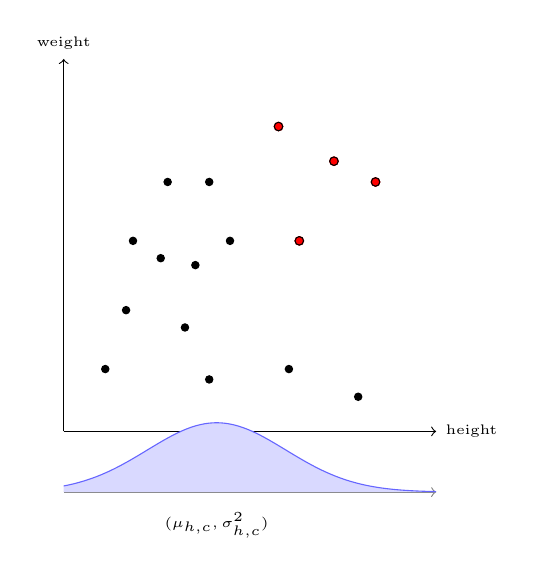
\begin{tikzpicture}[scale=0.55]
\draw[->] (0,0) -- (8.6,0) node[right]{\tiny height};
\draw[->] (0,0) -- (0,8.6) node[above]{\tiny weight};
\foreach \p in {(2.4,5.76),(3.36,5.76),(1.6,4.4),(2.24,4.0),(3.04,3.84),(3.84,4.4),(1.44,2.8),(2.8,2.4),(0.96,1.44),(3.36,1.2),(5.2,1.44),(6.8,0.8)}
\filldraw[black] \p circle (2.4pt);
\foreach \p in {(4.96,7.04),(6.24,6.24),(7.2,5.76),(5.44,4.4)}
{\filldraw[red] \p circle (2.8pt); \draw[black] \p circle (2.8pt);}
\begin{scope}[yshift=-1.4cm]
\draw[gray,->] (0,0) -- (8.6,0);
\fill[blue!15,domain=0:8.6,samples=60] plot (\x,{1.6*exp(-((\x-3.53)*(\x-3.53))/(2*1.6*1.6))}) -- (8.6,0) -- (0,0) -- cycle;
\draw[blue!60,domain=0:8.6,samples=60,smooth] plot (\x,{1.6*exp(-((\x-3.53)*(\x-3.53))/(2*1.6*1.6))});
\node[below] at (3.53,-0.25) {\tiny $(\mu_{h,c},\sigma^2_{h,c})$};
\end{scope}
\end{tikzpicture}
\end{adjustbox}
\end{center}
\tiny{Fit a Gaussian to that histogram; not a perfect fit, but easy to work with.}
\end{minipage}%
}

\begin{itemize}
\item Left: one child is really tall, the rest cluster on smaller values.
\item Right: the smooth Gaussian curve summarizes that histogram with just two numbers, its mean and standard deviation.
\end{itemize}
\end{frame}

% Merged (deck-review pass): "Adding Weight" + "Children Contour Plot" were two single-image
% frames making one continuous point (do the same for Weight, then combine both).
%%%%%%%%%%%%%%%%%%%%%%%%%%%%%%%%%%%%%%%%%%%%%%%%%%%%%%%%%%
\begin{frame}[fragile]\frametitle{Continuous Variable Example: Adding Weight, Then Combining Both}

\adjustbox{valign=t}{%
\begin{minipage}{0.47\linewidth}
\begin{center}
% 
\includegraphics[width=\linewidth,keepaspectratio]{nb15} -- too fuzzy at slide size; redrawn natively below.
\begin{adjustbox}{max width=\linewidth}
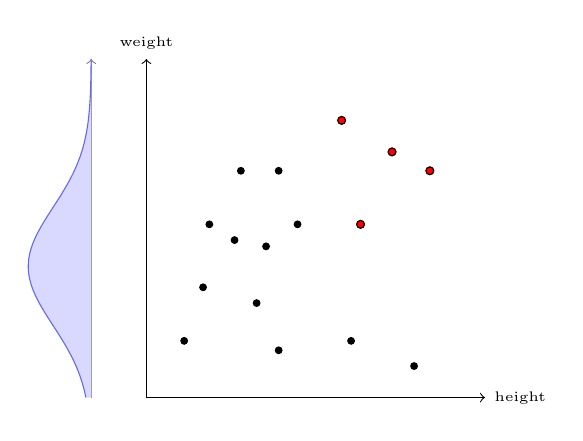
\begin{tikzpicture}[scale=0.5]
\draw[->] (0,0) -- (8.6,0) node[right]{\tiny height};
\draw[->] (0,0) -- (0,8.6) node[above]{\tiny weight};
\foreach \p in {(2.4,5.76),(3.36,5.76),(1.6,4.4),(2.24,4.0),(3.04,3.84),(3.84,4.4),(1.44,2.8),(2.8,2.4),(0.96,1.44),(3.36,1.2),(5.2,1.44),(6.8,0.8)}
\filldraw[black] \p circle (2.4pt);
\foreach \p in {(4.96,7.04),(6.24,6.24),(7.2,5.76),(5.44,4.4)}
{\filldraw[red] \p circle (2.8pt); \draw[black] \p circle (2.8pt);}
\begin{scope}[xshift=-1.4cm]
\draw[gray,->] (0,0) -- (0,8.6);
\fill[blue!15,domain=0:8.6,samples=60] plot ({-1.6*exp(-((\x-3.33)*(\x-3.33))/(2*1.5*1.5))},\x) -- (0,8.6) -- (0,0) -- cycle;
\draw[blue!60,domain=0:8.6,samples=60,smooth] plot ({-1.6*exp(-((\x-3.33)*(\x-3.33))/(2*1.5*1.5))},\x);
\end{scope}
\end{tikzpicture}
\end{adjustbox}
\end{center}
\tiny{The same Gaussian fit, done independently for Weight.}
\end{minipage}%
}%
\hfill%
\adjustbox{valign=t}{%
\begin{minipage}{0.47\linewidth}
\begin{center}
% 
\includegraphics[width=\linewidth,keepaspectratio]{nb17} -- too fuzzy at slide size; redrawn natively below.
\begin{adjustbox}{max width=\linewidth}
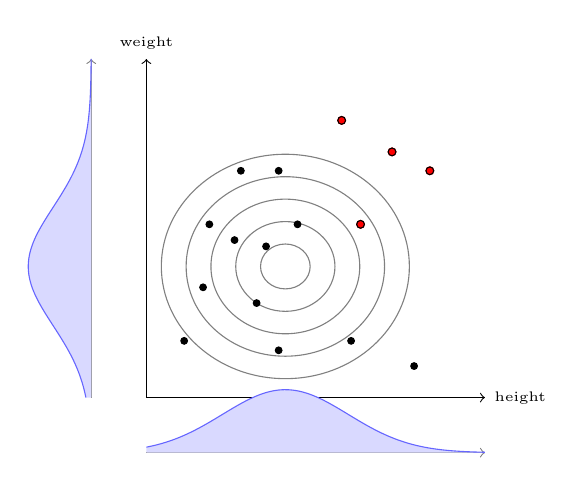
\begin{tikzpicture}[scale=0.5]
\draw[->] (0,0) -- (8.6,0) node[right]{\tiny height};
\draw[->] (0,0) -- (0,8.6) node[above]{\tiny weight};
\foreach \k in {0.6,1.2,1.8,2.4,3.0}
\draw[gray] (3.53,3.33) ellipse ({\k*1.05} and {\k*0.95});
\foreach \p in {(2.4,5.76),(3.36,5.76),(1.6,4.4),(2.24,4.0),(3.04,3.84),(3.84,4.4),(1.44,2.8),(2.8,2.4),(0.96,1.44),(3.36,1.2),(5.2,1.44),(6.8,0.8)}
\filldraw[black] \p circle (2.4pt);
\foreach \p in {(4.96,7.04),(6.24,6.24),(7.2,5.76),(5.44,4.4)}
{\filldraw[red] \p circle (2.8pt); \draw[black] \p circle (2.8pt);}
\begin{scope}[xshift=-1.4cm]
\draw[gray,->] (0,0) -- (0,8.6);
\fill[blue!15,domain=0:8.6,samples=60] plot ({-1.6*exp(-((\x-3.33)*(\x-3.33))/(2*1.5*1.5))},\x) -- (0,8.6) -- (0,0) -- cycle;
\draw[blue!60,domain=0:8.6,samples=60,smooth] plot ({-1.6*exp(-((\x-3.33)*(\x-3.33))/(2*1.5*1.5))},\x);
\end{scope}
\begin{scope}[yshift=-1.4cm]
\draw[gray,->] (0,0) -- (8.6,0);
\fill[blue!15,domain=0:8.6,samples=60] plot (\x,{1.6*exp(-((\x-3.53)*(\x-3.53))/(2*1.6*1.6))}) -- (8.6,0) -- (0,0) -- cycle;
\draw[blue!60,domain=0:8.6,samples=60,smooth] plot (\x,{1.6*exp(-((\x-3.53)*(\x-3.53))/(2*1.6*1.6))});
\end{scope}
\end{tikzpicture}
\end{adjustbox}
\end{center}
\tiny{Height and Weight combined into one 2D contour plot for Children; the peak is where both are near their typical values.}
\end{minipage}%
}

\begin{itemize}
\item Because the two Gaussians are assumed independent (the Naive Bayes assumption again, just for continuous features), their values can simply be multiplied together.
\end{itemize}
\end{frame}

%%%%%%%%%%%%%%%%%%%%%%%%%%%%%%%%%%%%%%%%%%%%%%%%%%%%%%%%%%
\begin{frame}[fragile]\frametitle{Continuous Variable Example: Adding the Adult Class}
\begin{itemize}
\item Adding Gaussian plot for Adults as well
\item You can start seeing separate regions, ie classification.
\item Thats the Gaussian Naive Bayes model
\end{itemize}
\begin{center}
% 
\includegraphics[width=0.5\linewidth,keepaspectratio]{nb18} -- too fuzzy at slide size; redrawn natively below.
\begin{adjustbox}{max width=0.58\linewidth}
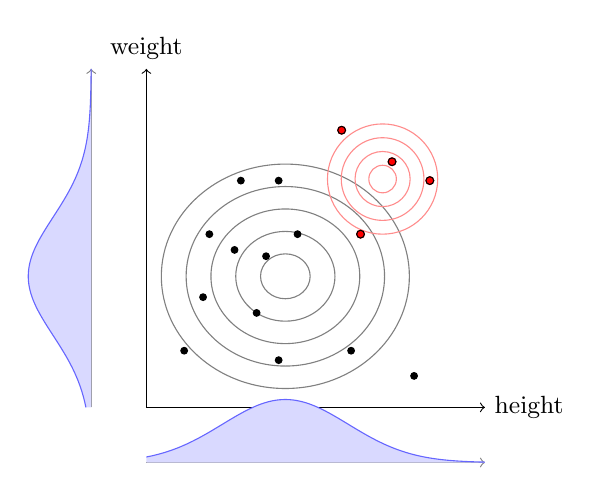
\begin{tikzpicture}[scale=0.5]
\draw[->] (0,0) -- (8.6,0) node[right]{\small height};
\draw[->] (0,0) -- (0,8.6) node[above]{\small weight};
\foreach \k in {0.6,1.2,1.8,2.4,3.0}
\draw[gray] (3.53,3.33) ellipse ({\k*1.05} and {\k*0.95});
\foreach \k in {0.35,0.7,1.05,1.4}
\draw[red!45] (6.0,5.8) ellipse ({\k*1.0} and {\k*1.0});
\foreach \p in {(2.4,5.76),(3.36,5.76),(1.6,4.4),(2.24,4.0),(3.04,3.84),(3.84,4.4),(1.44,2.8),(2.8,2.4),(0.96,1.44),(3.36,1.2),(5.2,1.44),(6.8,0.8)}
\filldraw[black] \p circle (2.4pt);
\foreach \p in {(4.96,7.04),(6.24,6.24),(7.2,5.76),(5.44,4.4)}
{\filldraw[red] \p circle (2.8pt); \draw[black] \p circle (2.8pt);}
\begin{scope}[xshift=-1.4cm]
\draw[gray,->] (0,0) -- (0,8.6);
\fill[blue!15,domain=0:8.6,samples=60] plot ({-1.6*exp(-((\x-3.33)*(\x-3.33))/(2*1.5*1.5))},\x) -- (0,8.6) -- (0,0) -- cycle;
\draw[blue!60,domain=0:8.6,samples=60,smooth] plot ({-1.6*exp(-((\x-3.33)*(\x-3.33))/(2*1.5*1.5))},\x);
\end{scope}
\begin{scope}[yshift=-1.4cm]
\draw[gray,->] (0,0) -- (8.6,0);
\fill[blue!15,domain=0:8.6,samples=60] plot (\x,{1.6*exp(-((\x-3.53)*(\x-3.53))/(2*1.6*1.6))}) -- (8.6,0) -- (0,0) -- cycle;
\draw[blue!60,domain=0:8.6,samples=60,smooth] plot (\x,{1.6*exp(-((\x-3.53)*(\x-3.53))/(2*1.6*1.6))});
\end{scope}
\end{tikzpicture}
\end{adjustbox}
\end{center}
\end{frame}

% Merged (deck-review pass): "Classifying a Test Point" + "The Final Classification" combined,
% and explanatory bullets added below the nb19 image (previously shown with zero surrounding
% text) so the six stacked formulas are read as a step-by-step recipe, not a wall of maths.
% Split into two frames (compile check, 2026-09-11): one frame with both the two intro bullets,
% the full-size image, and the four-step + winner bullets caused a 67pt overfull vbox that cut
% off the bottom bullet visibly on render -- too much content for one slide, not a spacing tweak.
% Both frames' nb19 screenshot replaced with the same native TikZ diagram (2026-09-11 pass) --
% too fuzzy to read at slide size, especially the six stacked formulas that used to be baked
% into the image; those are already covered in words by the bullets on the second frame.
%%%%%%%%%%%%%%%%%%%%%%%%%%%%%%%%%%%%%%%%%%%%%%%%%%%%%%%%%%
\begin{frame}[fragile]\frametitle{Continuous Variable Example: Classifying a New Point}
\begin{itemize}
\item A test point (the blue $\times$ below) has its own height and weight.
\item Plug both values into the Height-Gaussian and the Weight-Gaussian, separately for the Adult class and the Child class.
\end{itemize}
\begin{center}
% 
\includegraphics[width=0.7\linewidth,keepaspectratio]{nb19} -- too fuzzy at slide size; redrawn natively below.
\begin{adjustbox}{max width=0.62\linewidth}
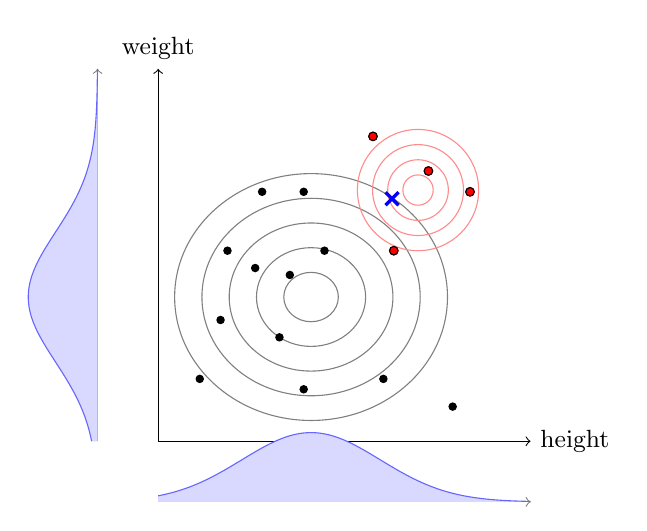
\begin{tikzpicture}[scale=0.55]
\draw[->] (0,0) -- (8.6,0) node[right]{\small height};
\draw[->] (0,0) -- (0,8.6) node[above]{\small weight};
\foreach \k in {0.6,1.2,1.8,2.4,3.0}
\draw[gray] (3.53,3.33) ellipse ({\k*1.05} and {\k*0.95});
\foreach \k in {0.35,0.7,1.05,1.4}
\draw[red!45] (6.0,5.8) ellipse ({\k*1.0} and {\k*1.0});
\foreach \p in {(2.4,5.76),(3.36,5.76),(1.6,4.4),(2.24,4.0),(3.04,3.84),(3.84,4.4),(1.44,2.8),(2.8,2.4),(0.96,1.44),(3.36,1.2),(5.2,1.44),(6.8,0.8)}
\filldraw[black] \p circle (2.4pt);
\foreach \p in {(4.96,7.04),(6.24,6.24),(7.2,5.76),(5.44,4.4)}
{\filldraw[red] \p circle (2.8pt); \draw[black] \p circle (2.8pt);}
\draw[blue,very thick] (5.25,5.45) -- (5.55,5.75);
\draw[blue,very thick] (5.25,5.75) -- (5.55,5.45);
\begin{scope}[xshift=-1.4cm]
\draw[gray,->] (0,0) -- (0,8.6);
\fill[blue!15,domain=0:8.6,samples=60] plot ({-1.6*exp(-((\x-3.33)*(\x-3.33))/(2*1.5*1.5))},\x) -- (0,8.6) -- (0,0) -- cycle;
\draw[blue!60,domain=0:8.6,samples=60,smooth] plot ({-1.6*exp(-((\x-3.33)*(\x-3.33))/(2*1.5*1.5))},\x);
\end{scope}
\begin{scope}[yshift=-1.4cm]
\draw[gray,->] (0,0) -- (8.6,0);
\fill[blue!15,domain=0:8.6,samples=60] plot (\x,{1.6*exp(-((\x-3.53)*(\x-3.53))/(2*1.6*1.6))}) -- (8.6,0) -- (0,0) -- cycle;
\draw[blue!60,domain=0:8.6,samples=60,smooth] plot (\x,{1.6*exp(-((\x-3.53)*(\x-3.53))/(2*1.6*1.6))});
\end{scope}
\end{tikzpicture}
\end{adjustbox}
\end{center}
\end{frame}

%%%%%%%%%%%%%%%%%%%%%%%%%%%%%%%%%%%%%%%%%%%%%%%%%%%%%%%%%%
\begin{frame}[fragile]\frametitle{Continuous Variable Example: Reading the Result}
\begin{center}
% 
\includegraphics[width=0.45\linewidth,keepaspectratio]{nb19} -- too fuzzy at slide size; redrawn natively below.
\begin{adjustbox}{max width=0.4\linewidth}
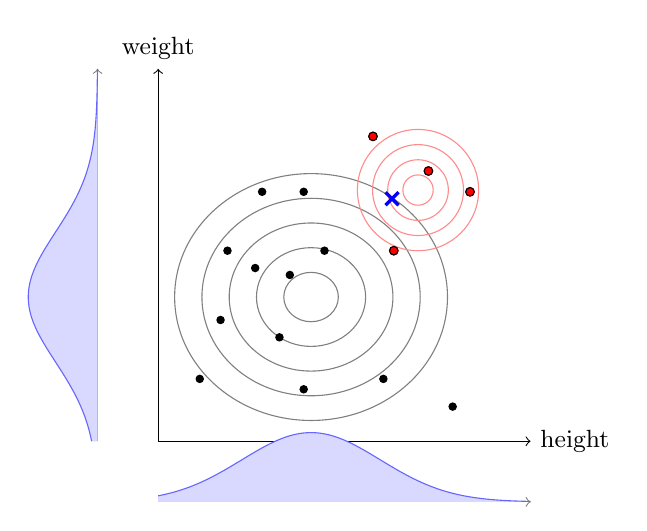
\begin{tikzpicture}[scale=0.55]
\draw[->] (0,0) -- (8.6,0) node[right]{\small height};
\draw[->] (0,0) -- (0,8.6) node[above]{\small weight};
\foreach \k in {0.6,1.2,1.8,2.4,3.0}
\draw[gray] (3.53,3.33) ellipse ({\k*1.05} and {\k*0.95});
\foreach \k in {0.35,0.7,1.05,1.4}
\draw[red!45] (6.0,5.8) ellipse ({\k*1.0} and {\k*1.0});
\foreach \p in {(2.4,5.76),(3.36,5.76),(1.6,4.4),(2.24,4.0),(3.04,3.84),(3.84,4.4),(1.44,2.8),(2.8,2.4),(0.96,1.44),(3.36,1.2),(5.2,1.44),(6.8,0.8)}
\filldraw[black] \p circle (2.4pt);
\foreach \p in {(4.96,7.04),(6.24,6.24),(7.2,5.76),(5.44,4.4)}
{\filldraw[red] \p circle (2.8pt); \draw[black] \p circle (2.8pt);}
\draw[blue,very thick] (5.25,5.45) -- (5.55,5.75);
\draw[blue,very thick] (5.25,5.75) -- (5.55,5.45);
\begin{scope}[xshift=-1.4cm]
\draw[gray,->] (0,0) -- (0,8.6);
\fill[blue!15,domain=0:8.6,samples=60] plot ({-1.6*exp(-((\x-3.33)*(\x-3.33))/(2*1.5*1.5))},\x) -- (0,8.6) -- (0,0) -- cycle;
\draw[blue!60,domain=0:8.6,samples=60,smooth] plot ({-1.6*exp(-((\x-3.33)*(\x-3.33))/(2*1.5*1.5))},\x);
\end{scope}
\begin{scope}[yshift=-1.4cm]
\draw[gray,->] (0,0) -- (8.6,0);
\fill[blue!15,domain=0:8.6,samples=60] plot (\x,{1.6*exp(-((\x-3.53)*(\x-3.53))/(2*1.6*1.6))}) -- (8.6,0) -- (0,0) -- cycle;
\draw[blue!60,domain=0:8.6,samples=60,smooth] plot (\x,{1.6*exp(-((\x-3.53)*(\x-3.53))/(2*1.6*1.6))});
\end{scope}
\end{tikzpicture}
\end{adjustbox}
\end{center}
\begin{itemize}
\item Read it as four steps: (1) each class's prior, $P(a)$ and $P(c)$; (2) each feature's likelihood given the class, e.g. $p(h_x|c)$ and $p(w_x|c)$; (3) multiply the two likelihoods within a class to get $P(x|\text{class})$; (4) combine with Bayes' rule to get $P(a|x)$ and $P(c|x)$.
\item Whichever class comes out with the bigger final probability wins, exactly the same recipe as the discrete Fruit example, just with Gaussian likelihoods in place of counted fractions.
\end{itemize}
\end{frame}






%%%%%%%%%%%%%%%%%%%%%%%%%%%%%%%%%%%%%%%%%%%%%%%%%%%%%%%%%%
\begin{frame}[fragile]\frametitle{Quick Check: Naive Bayes}
\begin{block}{Think About It}
In the rare-disease example, most of the probability mass ended up on ``no disease'' even
though the test came back positive, despite the test being 97-98\% accurate. Why does a low
base rate (prior) ``defeat'' a seemingly accurate test, and what does this imply about
interpreting positive results for rare conditions in general?
\end{block}
\end{frame}

%%%%%%%%%%%%%%%%%%%%%%%%%%%%%%%%%%%%%%%%%%%%%%%%%%%%%%%%%%%%%%%%%%%%%%%%%%%%%%%%%%
\begin{frame}[fragile]\frametitle{Quick Check: Naive Bayes}
\begin{block}{Answer}
Because the healthy population is so much larger than the sick population, even a small
false-positive rate applied to that huge healthy group produces more false alarms than true
positives from the tiny sick group. This is the base-rate fallacy: a test's accuracy
percentage alone never tells you the probability of disease given a positive result, you
must always weigh it against the prior, exactly what Bayes' Theorem forces you to do.
\end{block}
\end{frame}

%%%%%%%%%%%%%%%%%%%%%%%%%%%%%%%%%%%%%%%%%%%%%%%%%%%%%%%%%
\begin{frame}[fragile]\frametitle{Pros and cons}
Advantages
\begin{itemize}
\item     It's relatively simple to understand and build
\item     It's easily trained, even with a small data-set
\item     It's fast!
\item     It's not sensitive to irrelevant features
\end{itemize}
Disadvantages
\begin{itemize}
\item     It assumes every feature is independent, which isn't always the case
\end{itemize}
\end{frame}




%%%%%%%%%%%%%%%%%%%%%%%%%%%%%%%%%%%%%%%%%%%%%%%%%%%%%%%%%%
\begin{frame}[fragile]\frametitle{Naive Bayes (Summary): Why It Works}
\begin{itemize}
\item Classification based on Bayes theorem
\item Assumption of independence between predictors.
\item That is a too `naive' assumption to make.
\item Naive Bayesian model is easy to build and particularly useful for very large data sets. 
\item Along with simplicity, Naive Bayes is known to outperform even highly sophisticated classification methods.
\end{itemize}
\end{frame}


%%%%%%%%%%%%%%%%%%%%%%%%%%%%%%%%%%%%%%%%%%%%%%%%%%%%%%%%%%
\begin{frame}[fragile]\frametitle{Naive Bayes (Summary): When It Struggles}
\begin{itemize}
\item In many datasets, relationship between attributes and class variable is non-deterministic.
\item Why?
	\begin{itemize}
	\item Noisy data
	\item Confounding and interaction of factors
	\item Relevant variables not included in the data
	\end{itemize}

\item Scenario
	\begin{itemize}
	\item Risk of heart disease based on individual's diet and workout frequency
	\item Most people who ``work out'' and have a healthy diet don't get heart disease. Yet, some healthy individuals still do: Smoking, alcohol abuse
	\end{itemize}
\end{itemize}
\end{frame}